% Options for packages loaded elsewhere
\PassOptionsToPackage{unicode}{hyperref}
\PassOptionsToPackage{hyphens}{url}
\documentclass[
  brazilian,
]{article}
\usepackage{xcolor}
\usepackage[margin=2cm]{geometry}
\usepackage{amsmath,amssymb}
\setcounter{secnumdepth}{5}
\usepackage{iftex}
\ifPDFTeX
  \usepackage[T1]{fontenc}
  \usepackage[utf8]{inputenc}
  \usepackage{textcomp} % provide euro and other symbols
\else % if luatex or xetex
  \usepackage{unicode-math} % this also loads fontspec
  \defaultfontfeatures{Scale=MatchLowercase}
  \defaultfontfeatures[\rmfamily]{Ligatures=TeX,Scale=1}
\fi
\usepackage{lmodern}
\ifPDFTeX\else
  % xetex/luatex font selection
  \setmainfont[]{Times New Roman}
\fi
% Use upquote if available, for straight quotes in verbatim environments
\IfFileExists{upquote.sty}{\usepackage{upquote}}{}
\IfFileExists{microtype.sty}{% use microtype if available
  \usepackage[]{microtype}
  \UseMicrotypeSet[protrusion]{basicmath} % disable protrusion for tt fonts
}{}
\makeatletter
\@ifundefined{KOMAClassName}{% if non-KOMA class
  \IfFileExists{parskip.sty}{%
    \usepackage{parskip}
  }{% else
    \setlength{\parindent}{0pt}
    \setlength{\parskip}{6pt plus 2pt minus 1pt}}
}{% if KOMA class
  \KOMAoptions{parskip=half}}
\makeatother
\usepackage{longtable,booktabs,array}
\newcounter{none} % for unnumbered tables
\usepackage{calc} % for calculating minipage widths
% Correct order of tables after \paragraph or \subparagraph
\usepackage{etoolbox}
\makeatletter
\patchcmd\longtable{\par}{\if@noskipsec\mbox{}\fi\par}{}{}
\makeatother
% Allow footnotes in longtable head/foot
\IfFileExists{footnotehyper.sty}{\usepackage{footnotehyper}}{\usepackage{footnote}}
\makesavenoteenv{longtable}
\usepackage{graphicx}
\makeatletter
\newsavebox\pandoc@box
\newcommand*\pandocbounded[1]{% scales image to fit in text height/width
  \sbox\pandoc@box{#1}%
  \Gscale@div\@tempa{\textheight}{\dimexpr\ht\pandoc@box+\dp\pandoc@box\relax}%
  \Gscale@div\@tempb{\linewidth}{\wd\pandoc@box}%
  \ifdim\@tempb\p@<\@tempa\p@\let\@tempa\@tempb\fi% select the smaller of both
  \ifdim\@tempa\p@<\p@\scalebox{\@tempa}{\usebox\pandoc@box}%
  \else\usebox{\pandoc@box}%
  \fi%
}
% Set default figure placement to htbp
\def\fps@figure{htbp}
\makeatother
\ifLuaTeX
\usepackage[bidi=basic,shorthands=off]{babel}
\else
\usepackage[bidi=default,shorthands=off]{babel}
\fi
\ifPDFTeX
\else
\babelfont{rm}[]{Times New Roman}
\fi
\ifLuaTeX
  \usepackage{selnolig} % disable illegal ligatures
\fi
\setlength{\emergencystretch}{3em} % prevent overfull lines
\providecommand{\tightlist}{%
  \setlength{\itemsep}{0pt}\setlength{\parskip}{0pt}}
\setlength{\LTleft}{0pt}
\setlength{\LTright}{0pt}
\setlength{\emergencystretch}{5em}
\AtBeginEnvironment{longtable}{\setlength{\tabcolsep}{3pt}\scriptsize}
\usepackage{caption}
\newcommand{\tablecaptionbelow}[1]{%
  \begin{center}
  \begin{minipage}{\linewidth}
  \captionof{table}{#1}
  \end{minipage}
  \end{center}}
\usepackage{placeins}
\let\oldunderscore\_
\renewcommand{\_}{\oldunderscore\discretionary{}{}{}}
\usepackage{bookmark}
\IfFileExists{xurl.sty}{\usepackage{xurl}}{} % add URL line breaks if available
\urlstyle{same}
\hypersetup{
  pdftitle={Relatório de Caracterização Experimental e Estatística do Estágio de Saída de um Estimulador Elétrico Funcional},
  pdfauthor={Tiago de Paula Silva},
  pdflang={pt-BR},
  hidelinks,
  pdfcreator={LaTeX via pandoc}}

\title{Relatório de Caracterização Experimental e Estatística do Estágio
de Saída de um Estimulador Elétrico Funcional}
\author{Tiago de Paula Silva}
\date{24 de maio de 2026}

\begin{document}
\maketitle

{
\setcounter{tocdepth}{3}
\tableofcontents
}
\section{Problema}\label{problema}

O item de estudo é o estágio de saída de um estimulador elétrico
funcional (FES) baseado em uma fonte de corrente Howland. Mais
especificamente, trata-se do eletroestimulador STIMGRASP, desenvolvido
por Renato Barelli em 2017 como parte de uma dissertação de mestrado.

Na dissertação de Renato Barelli, a arquitetura é apresentada e a
linearidade do estágio de saída é afirmada como característica esperada
do circuito, mas não é feita uma caracterização experimental
quantitativa dessa linearidade. Também não são avaliadas, de forma
sistemática, a dependência da corrente em relação à carga conectada nem
os limites de operação em tensão impostos pela arquitetura.

Nesta arquitetura, o microcontrolador define uma tensão de controle no
DAC, e essa tensão deve produzir uma corrente de saída previsível no
paciente ou em uma carga equivalente.

O problema central é que o circuito opera em malha aberta: o
microcontrolador não mede a corrente real entregue durante a operação.
Assim, se a carga mudar, se o contato eletrodo-pele piorar ou se o
circuito atingir seu limite de tensão de operação (voltage compliance),
a corrente entregue pode deixar de seguir o valor esperado. Como não há
realimentação de corrente, essa perda de previsibilidade não é detectada
diretamente pelo firmware do STIMGRASP.

Por isso, é necessário caracterizar experimentalmente a relação entre
tensão de DAC e corrente de saída, identificando a região em que o
circuito se comporta aproximadamente como fonte de corrente, a
influência da carga resistiva sobre a corrente entregue, um modelo
matemático útil para estimar a corrente a partir do DAC e evidências
estatísticas sobre linearidade, erro e limitação por compliance.

\section{Motivação}\label{motivauxe7uxe3o}

Em estimulação elétrica funcional, a amplitude de corrente está
associada à resposta neuromuscular, ao conforto do usuário e à
repetibilidade do protocolo de estimulação. Se a corrente real não for
previsível, o mesmo comando digital pode gerar respostas diferentes em
diferentes condições de carga.

Este relatório é inspirado no artigo \emph{Experimental Characterization
of the Output Stage of a Functional Electrical Stimulator Based on a
Howland Current Source}, produzido no contexto da disciplina PEL309
{[}1{]}. Naquele trabalho, com análise em Python, o STIMGRASP foi
caracterizado experimentalmente por meio da relação entre tensão de DAC
e corrente de saída, seleção da região de compliance, correlação e
regressão linear.

O presente relatório revisa e aprofunda essa caracterização em R, com
uma análise estatística mais cuidadosa para a disciplina PME406. A
versão atual prioriza a consistência estatística da caracterização: a
região útil é definida antes da regressão, os modelos são avaliados por
erro, resíduos, intervalos e validação cruzada, e análises multivariadas
ou didáticas são tratadas como material secundário quando não sustentam
diretamente a conclusão técnica.

\section{Objetivo}\label{objetivo}

O objetivo do script é executar uma análise estatística da relação entre
tensão de DAC e corrente de saída para três cargas resistivas nominais:
1 kOhm, 2 kOhm e 4,7 kOhm.

Seguindo a motivação apresentada no trabalho anterior, a análise é
organizada em três perguntas centrais:

\begin{itemize}
\tightlist
\item
  existe linearidade quantificável entre o sinal de controle do DAC e a
  corrente de saída na região válida de operação?
\item
  quais são os limites de tensão de operação do estágio de saída antes
  da limitação por compliance?
\item
  a relação DAC-corrente permanece consistente quando a carga resistiva
  muda?
\end{itemize}

Os objetivos específicos são:

\begin{itemize}
\tightlist
\item
  importar os dados experimentais do osciloscópio;
\item
  extrair a região útil da rampa de DAC;
\item
  converter tensão no resistor shunt em corrente de saída;
\item
  agregar os dados por bins de tensão de DAC;
\item
  identificar a região comum de compliance;
\item
  avaliar linearidade por correlação e regressão;
\item
  comparar o modelo global com o ajuste que considera a influência da
  carga na relação entre comando de DAC e corrente de saída;
\item
  quantificar erro de predição, resíduos e heterocedasticidade;
\item
  explicitar limitações de normalidade e independência dos resíduos.
\end{itemize}

\section{Estrutura da análise}\label{estrutura-da-anuxe1lise}

A análise que deu origem às tabelas e figuras deste relatório foi
implementada no script \texttt{analise\_rstudio.R}, disponível
publicamente no GitHub {[}2{]}:
\url{https://github.com/import-tiago/FEI/blob/main/MSc/PME406/1.Analysis/analise_rstudio.R}.
Esse script em R lê os CSVs exportados do osciloscópio, remove trechos
estacionários antes e depois da rampa útil, calcula corrente a partir da
tensão no resistor shunt, reconstrói a tensão na carga por resistência
nominal e agrega os dados por bins de DAC de 10 mV. Os dados brutos
utilizados como entrada da análise correspondem aos arquivos
\texttt{1k.csv}, \texttt{2k.csv} e \texttt{4k7.csv}, também disponíveis
no GitHub {[}3{]}.

O fluxo de análise segue a sequência: aquisição CSV do osciloscópio,
extração da rampa útil, conversão da tensão no shunt para corrente,
agregação por bins de DAC, seleção da região de compliance, regressão
linear, comparação entre modelos, análise dos resíduos e validação
cruzada por blocos.

A partir desse conjunto processado, o relatório seleciona a região comum
de compliance, ajusta modelos lineares, compara modelos aninhados por
ANOVA/teste F, calcula métricas de erro, examina resíduos, avalia
heterocedasticidade e verifica a estabilidade preditiva por validação
cruzada em blocos. Todas as tabelas são exportadas para a pasta
\texttt{tables}, e as figuras são exportadas para a pasta
\texttt{figures}.

\clearpage

\section{Desenho experimental, coleta e
limitações}\label{desenho-experimental-coleta-e-limitauxe7uxf5es}

Foram analisadas rampas de tensão de DAC e tensão no resistor shunt para
três cargas resistivas nominais: 1 kOhm, 2 kOhm e 4,7 kOhm. A análise
estima corrente a partir do shunt e reconstrói a tensão na carga por
resistência nominal. Como o sistema opera em malha aberta, a regressão
caracteriza o comportamento observado no ensaio, mas não garante
corrente entregue em operação real quando a carga, contato eletrodo-pele
ou condições térmicas mudam.

A coleta foi realizada com firmware experimental dedicado a gerar uma
rampa controlada de DAC. A tensão de controle foi medida no canal CH1 do
osciloscópio, enquanto a tensão associada à saída foi medida no canal
CH2 sobre o arranjo de carga e resistor shunt. O objetivo dessa
instrumentação foi caracterizar o estágio de saída, não representar uma
sessão completa de estimulação terapêutica.

\begin{center}
\begin{minipage}[t]{0.495\linewidth}
\centering
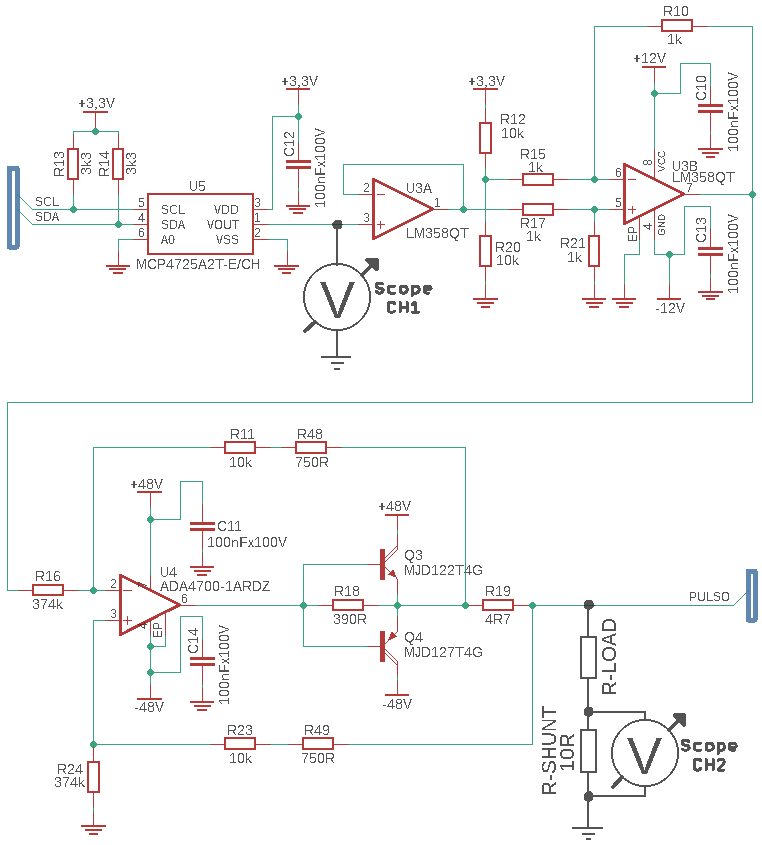
\includegraphics[width=\linewidth,keepaspectratio]{figures/00_output_stage_measurement_points.png}
\captionof{figure}{Estágio DAC/Howland do STIMGRASP com pontos de medição usados na coleta experimental}
\end{minipage}
\hfill
\begin{minipage}[t]{0.495\linewidth}
\centering
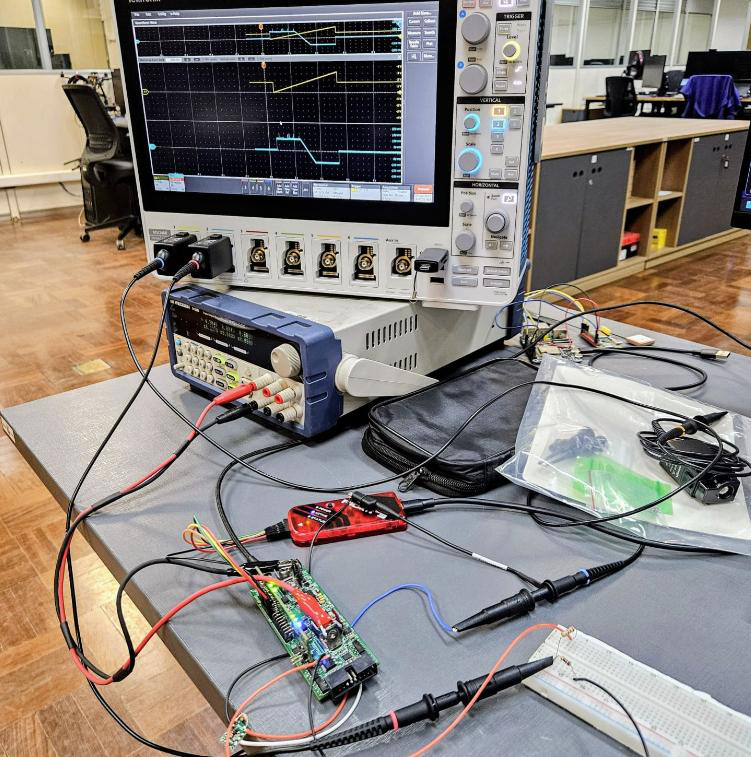
\includegraphics[width=\linewidth,keepaspectratio]{figures/00_data_collection_setup.png}
\captionof{figure}{Bancada experimental usada para aquisição dos sinais de DAC e shunt}
\end{minipage}
\end{center}
\clearpage

\section{Importação e
pré-processamento}\label{importauxe7uxe3o-e-pruxe9-processamento}

Os CSVs foram importados diretamente dos arquivos do osciloscópio,
removendo os segmentos estacionários antes e depois da rampa útil. As
três cargas foram equalizadas para a mesma quantidade de amostras.

Cada arquivo contém duas grandezas principais: \texttt{dac\_volts}, que
representa a tensão de controle aplicada ao estágio de saída, e
\texttt{shunt\_volts}, que representa a tensão medida no resistor shunt
e é usada para calcular a corrente.

Os dados brutos utilizados nesta etapa são os arquivos CSV
\texttt{1k.csv}, \texttt{2k.csv} e \texttt{4k7.csv}, disponíveis no
repositório indicado na Referência {[}3{]}.

Antes de qualquer tratamento, apenas como um exemplo, a carga de 1 kOhm
possui a seguinte prévia dos dados crus:

\begin{table}[htbp]
\centering
\makebox[\textwidth][c]{%
\begin{minipage}[t]{0.42\textwidth}
\vspace{0pt}
\centering
\scriptsize
\begin{tabular}{@{}lll@{}}
\toprule
Tensão DAC (V) & Tensão no shunt (V) & Amostra \\
\midrule
1.626406 & 0.002984 & 0 \\
1.628438 & 0.002797 & 1 \\
1.627500 & 0.001016 & 2 \\
1.628906 & 0.003047 & 3 \\
1.627031 & 0.005047 & 4 \\
\bottomrule
\end{tabular}
\end{minipage}%
\hspace{0.03\textwidth}%
\begin{minipage}[t]{0.18\textwidth}
\vspace{0pt}
\centering
\scriptsize
\begin{tabular}{@{}ll@{}}
\toprule
Carga & Amostras \\
\midrule
1k & 58386 \\
2k & 58386 \\
4k7 & 58386 \\
\bottomrule
\end{tabular}
\end{minipage}%
}
\caption{Prévia dos dados crus e quantidade de amostras por carga}
\end{table}
\FloatBarrier

\begin{center}
\captionsetup{font=small}
\begin{minipage}[t]{0.495\linewidth}
\centering
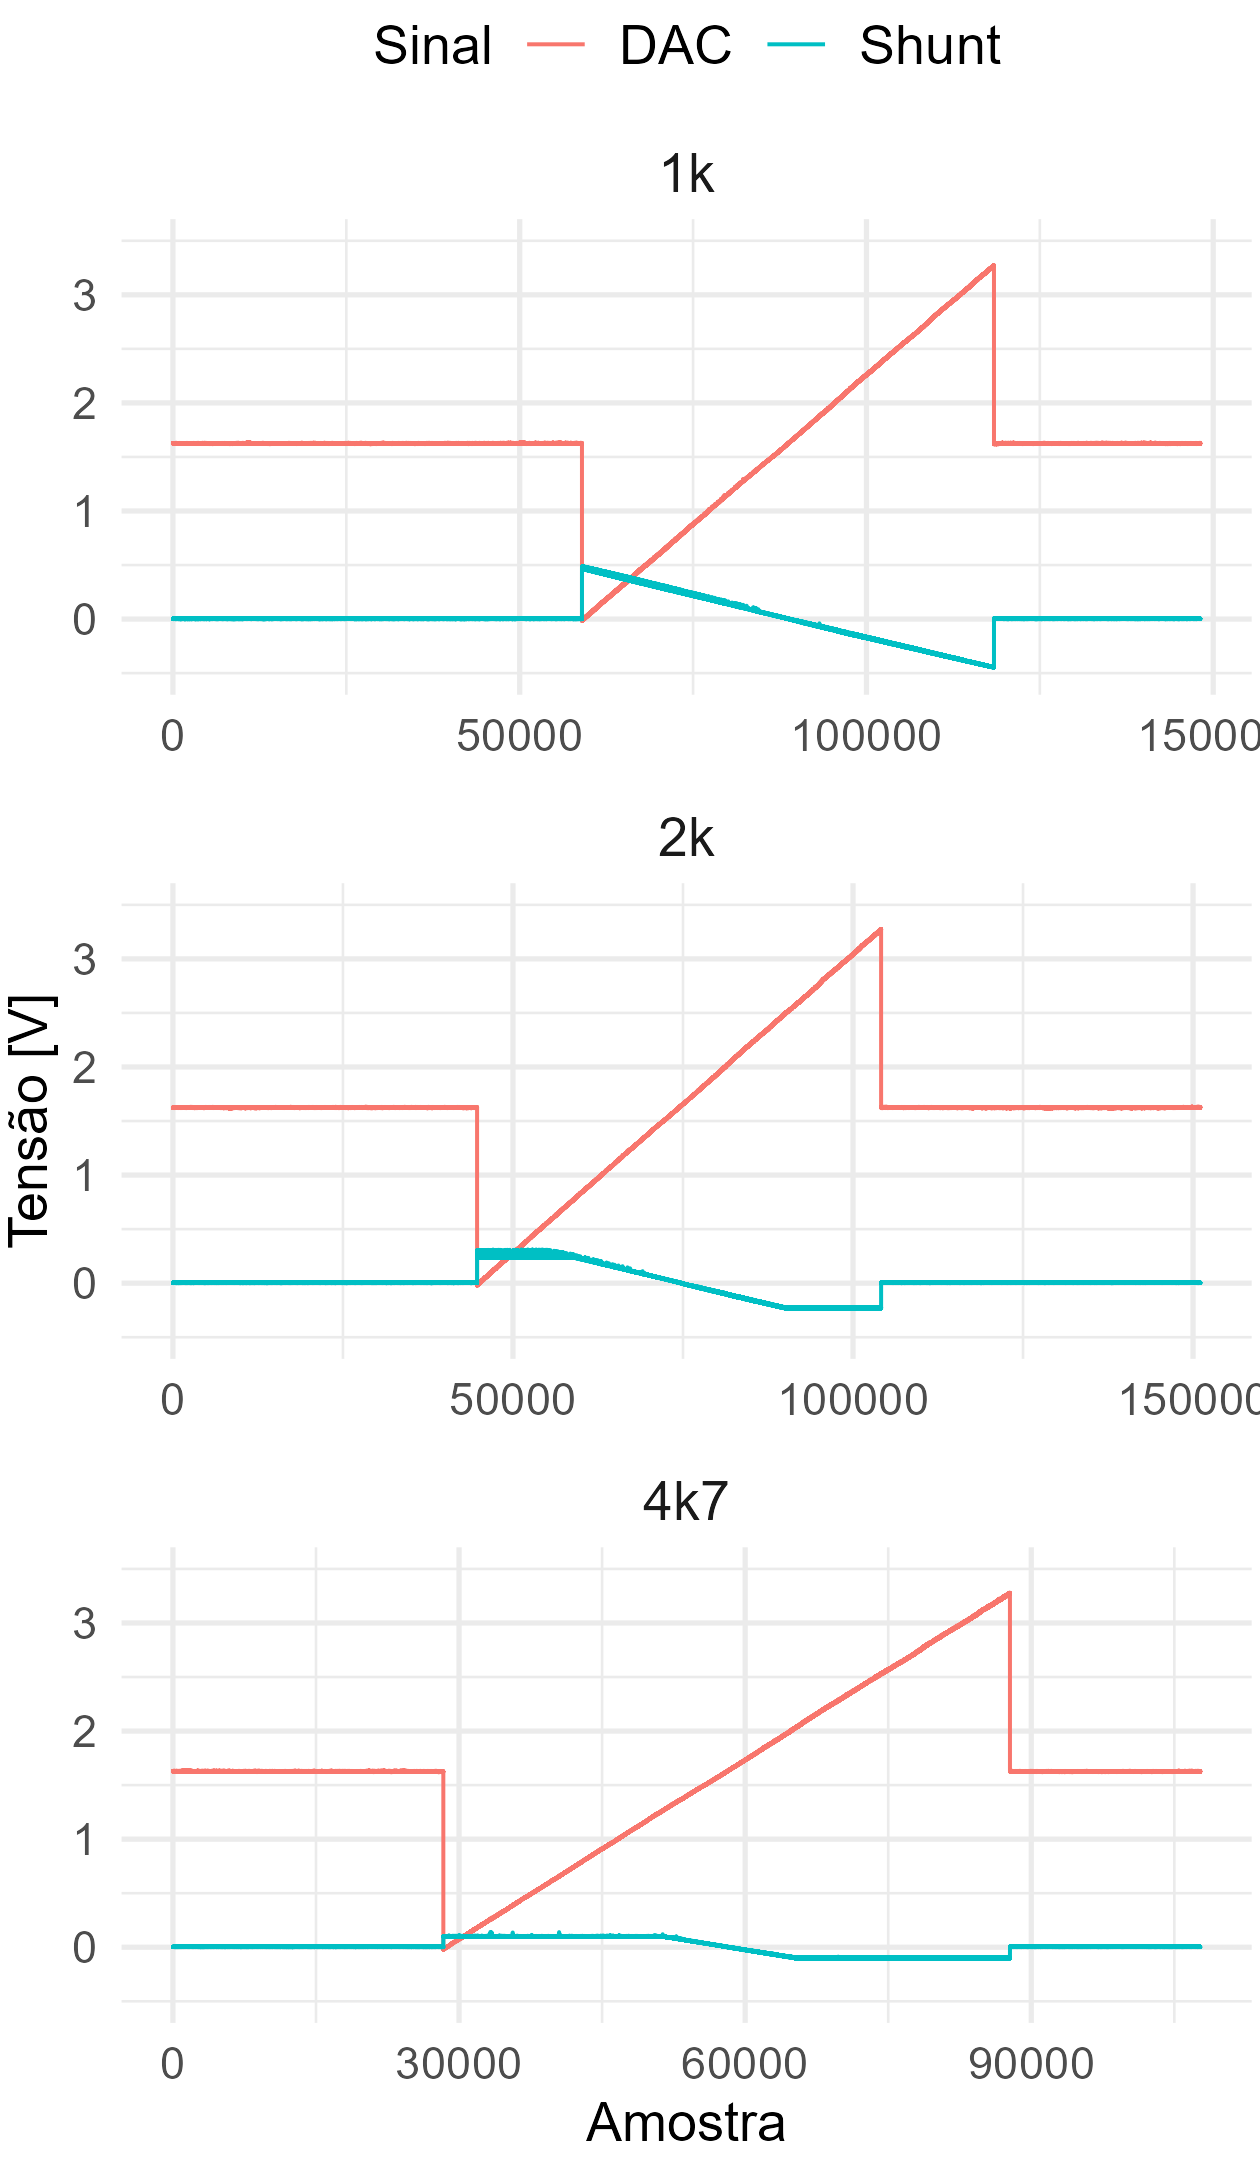
\includegraphics[width=\linewidth,keepaspectratio]{figures/01_raw_signals_before_stationary_removal.png}
\captionof{figure}{Sinais brutos antes da remoção dos segmentos estacionários}
\end{minipage}
\hfill
\begin{minipage}[t]{0.495\linewidth}
\centering
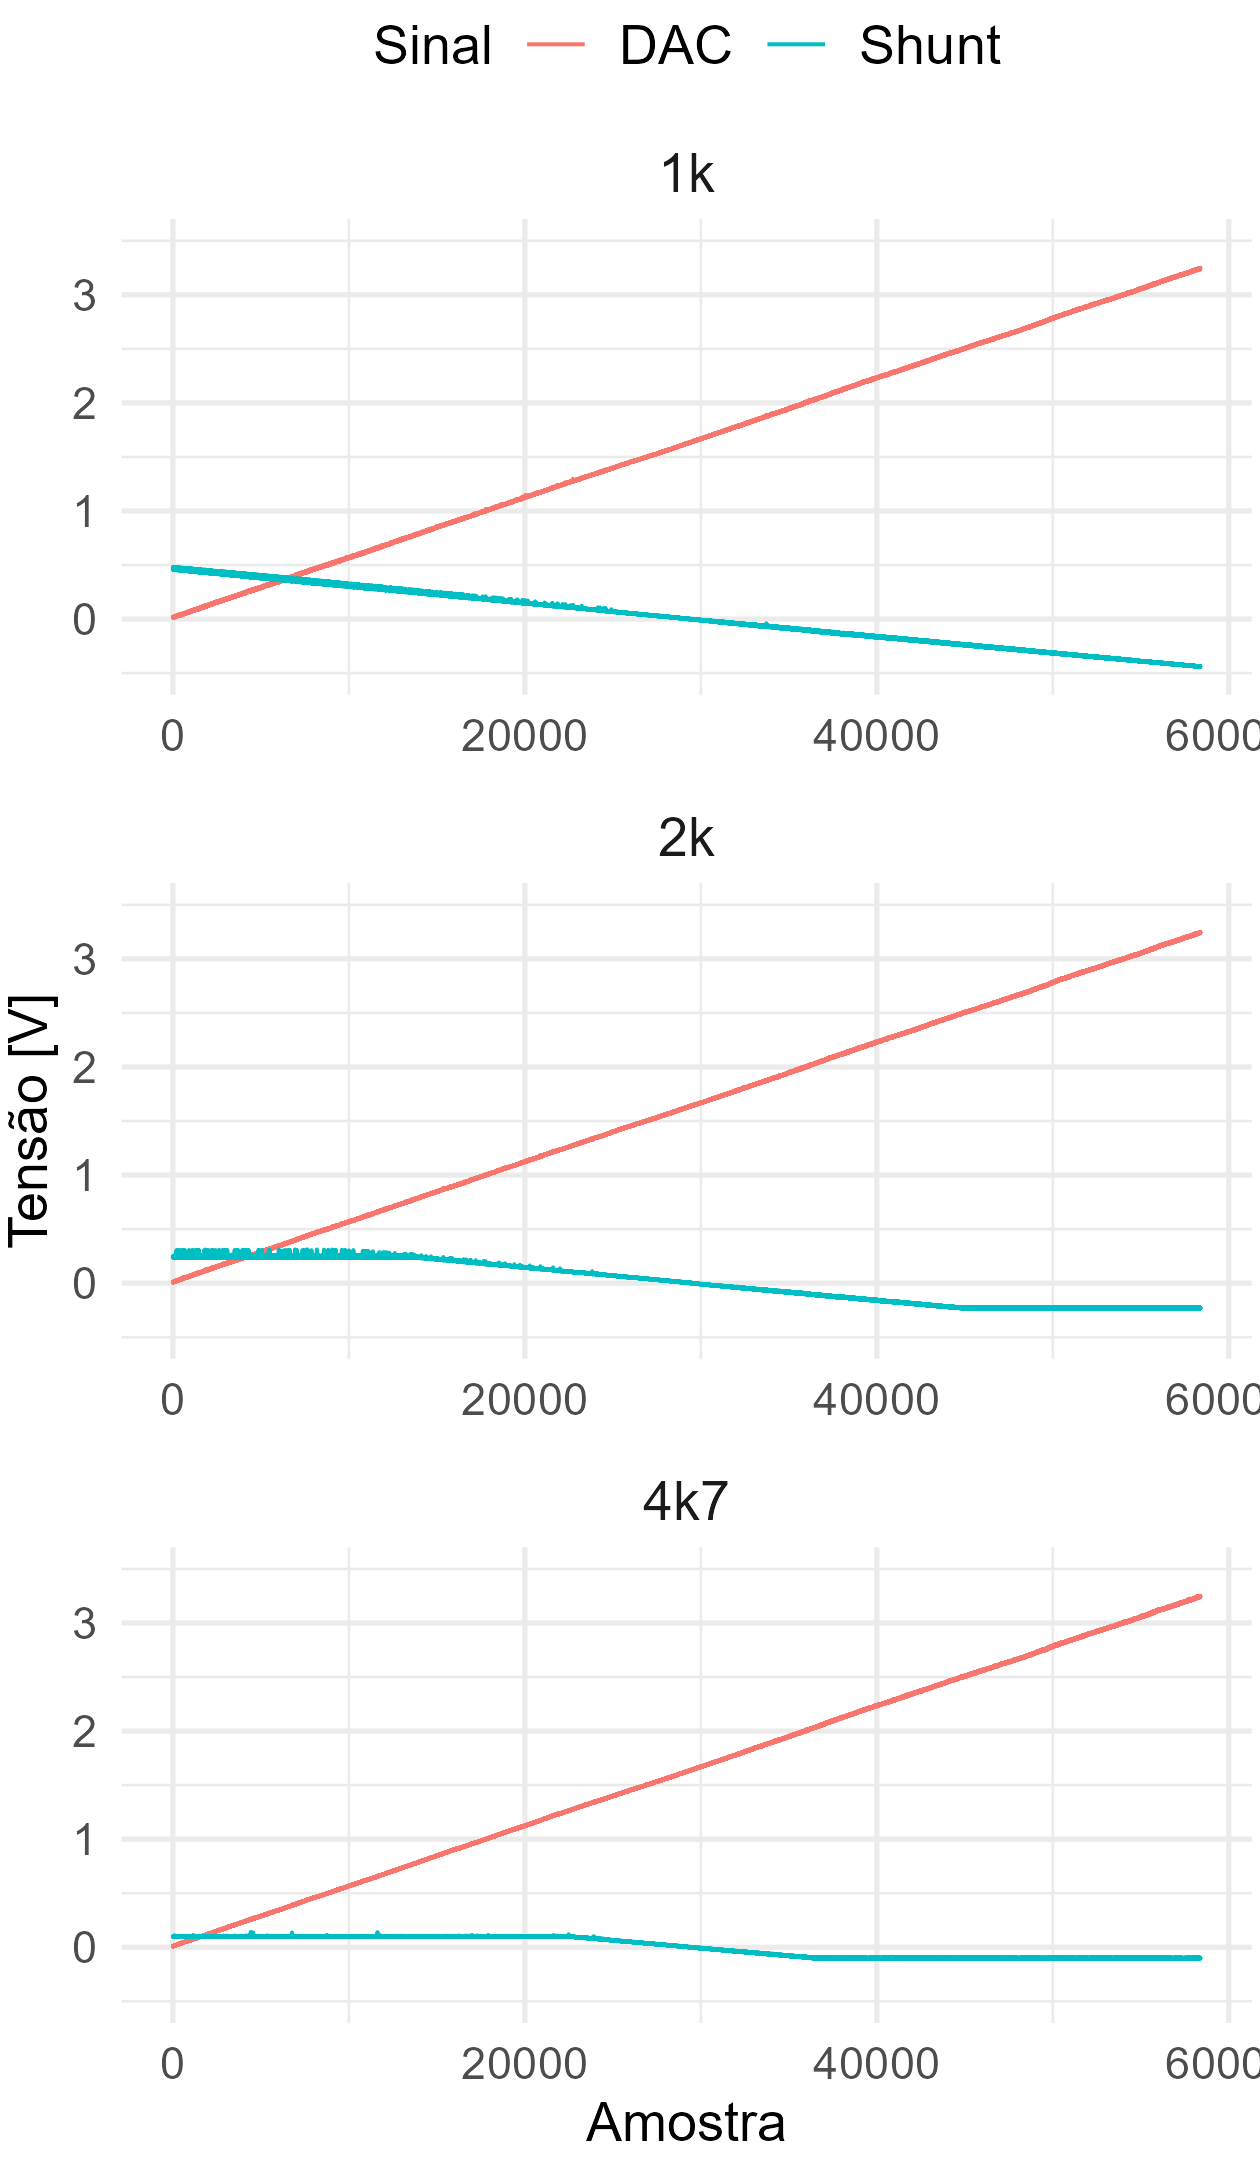
\includegraphics[width=\linewidth,keepaspectratio]{figures/02_ramp_signals_after_stationary_removal.png}
\captionof{figure}{Sinais da rampa após a remoção dos segmentos estacionários}
\end{minipage}
\end{center}
\FloatBarrier

\clearpage

\section{Conversão shunt-corrente}\label{conversuxe3o-shunt-corrente}

A corrente foi calculada a partir da tensão medida no resistor shunt,
conforme a Equação~\ref{eq:current-shunt}, com \(R_{\mathrm{shunt}} =
10\ \Omega\). A tolerância configurada do shunt é 1\%.
\begin{equation}
I = \frac{V_{\mathrm{shunt}}}{R_{\mathrm{shunt}}}
\label{eq:current-shunt}
\end{equation}

\begin{center}
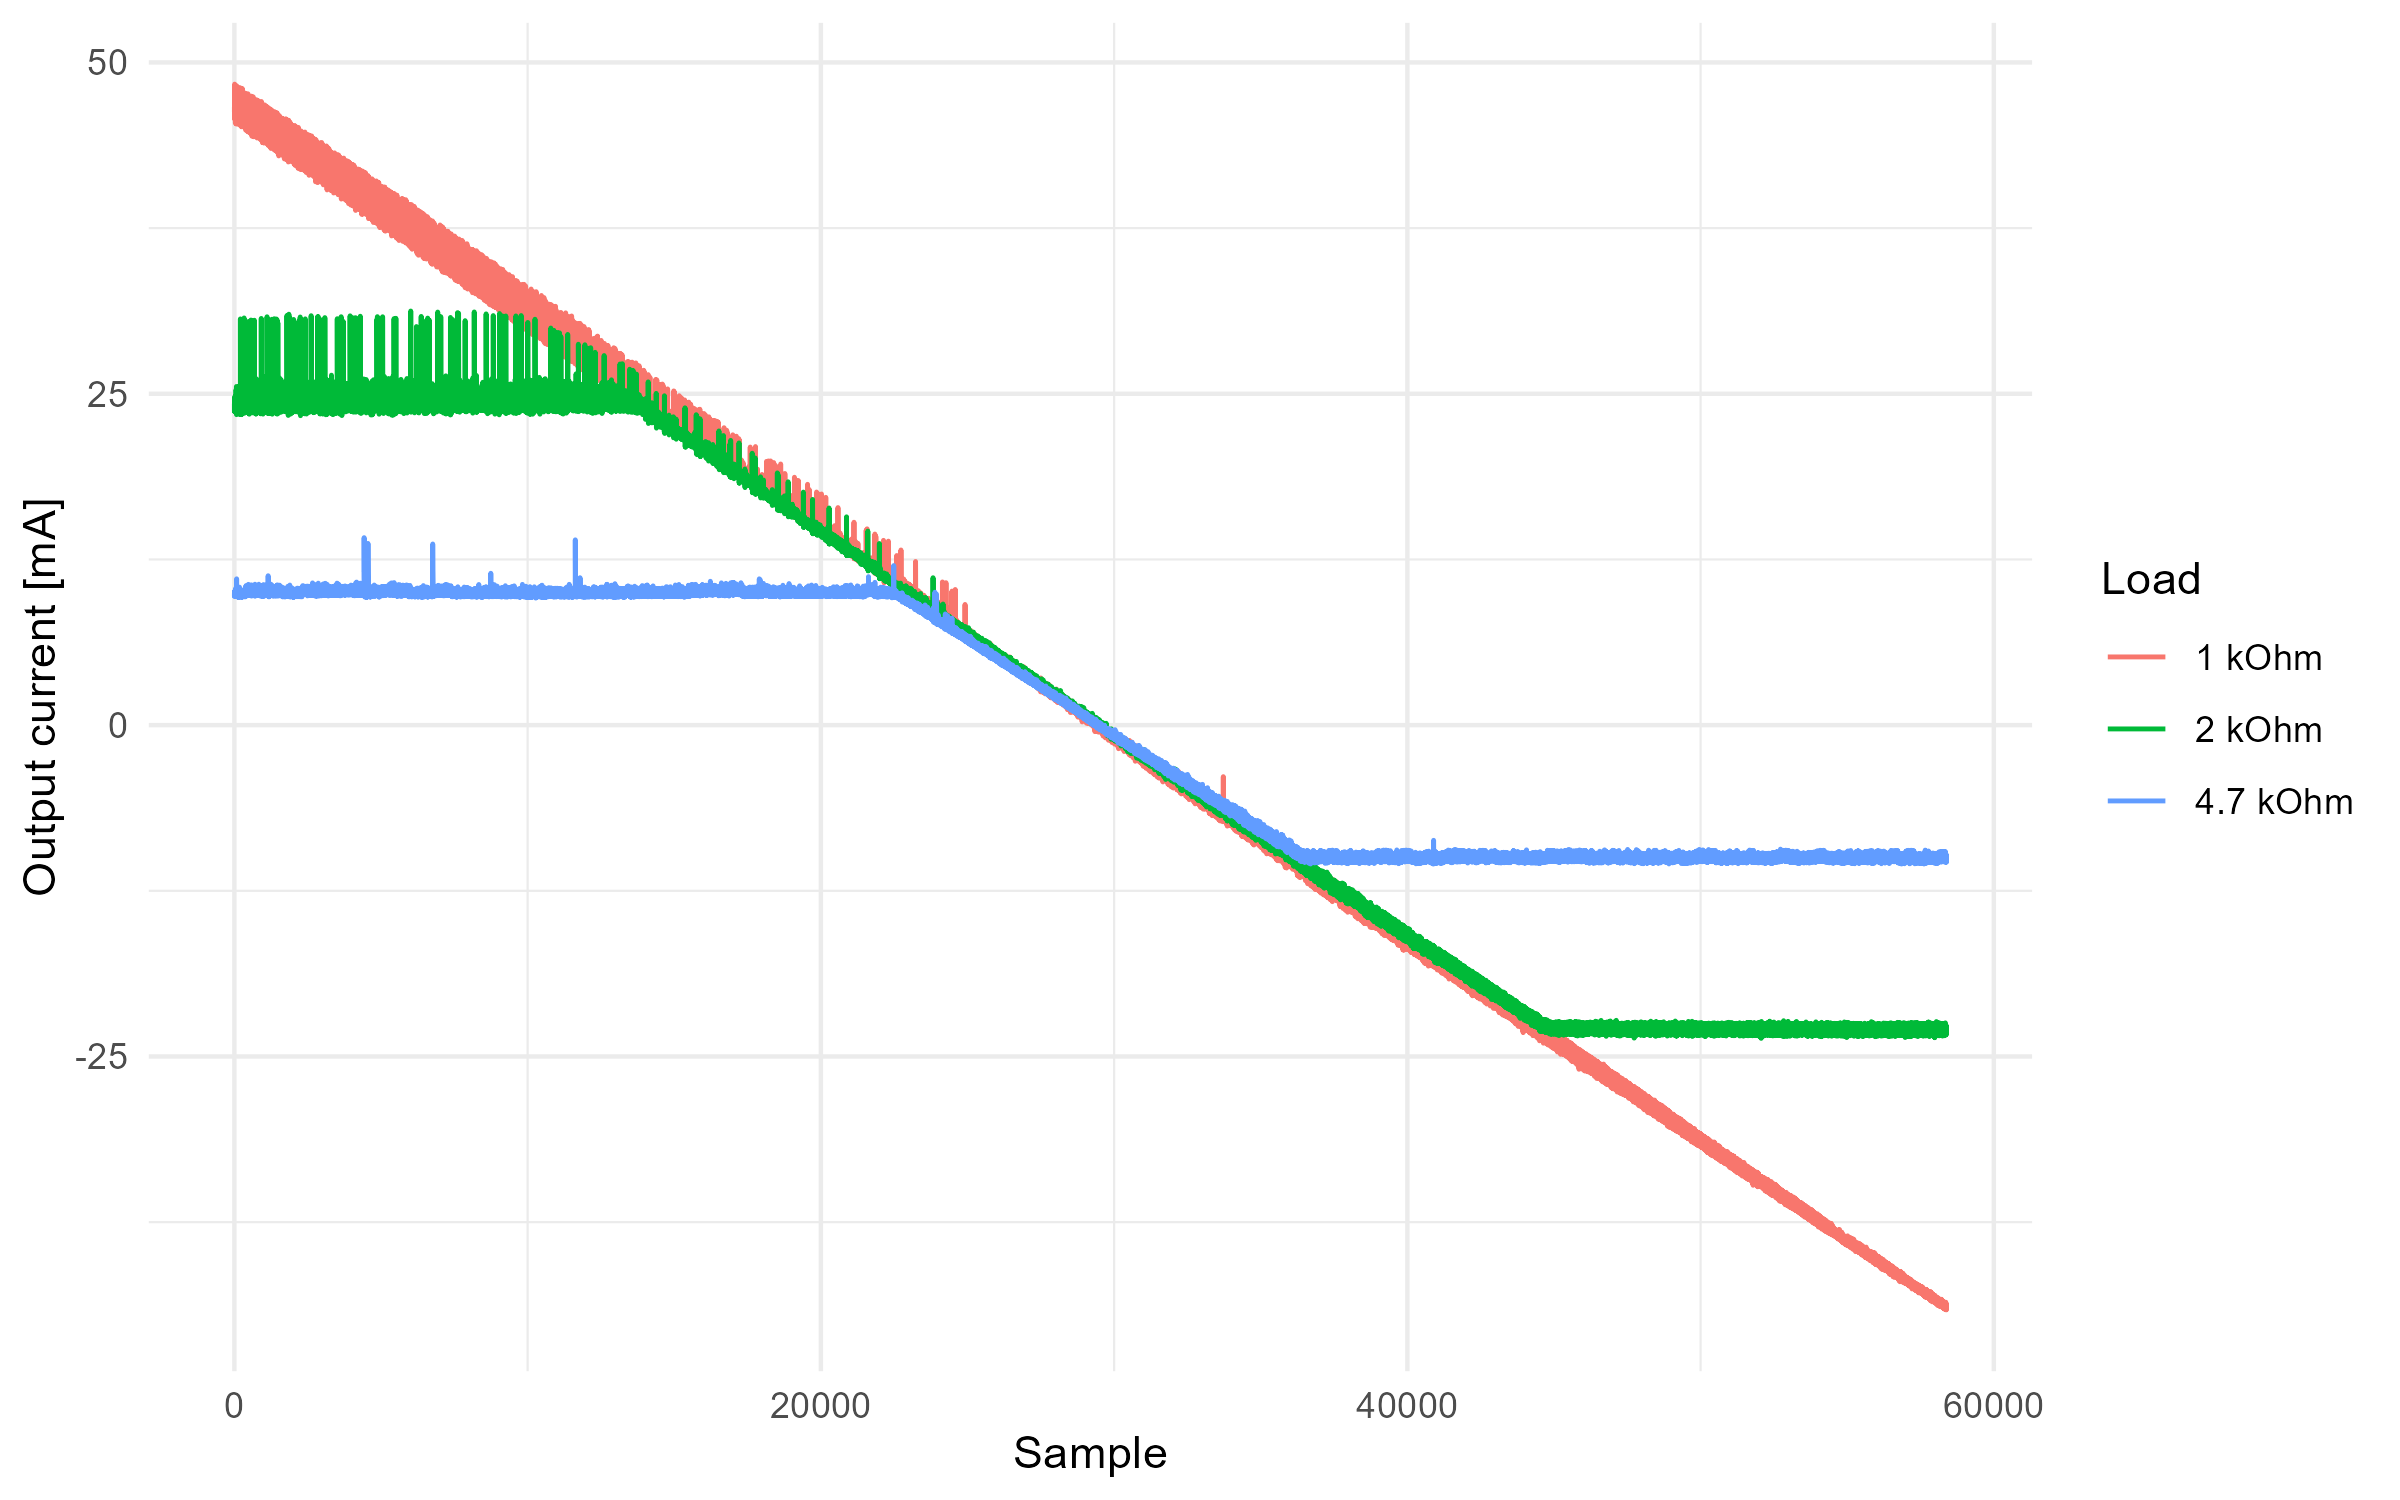
\includegraphics[width=0.78\linewidth,keepaspectratio]{figures/03_current_after_conversion.png}
\captionof{figure}{Corrente calculada após conversão da tensão no shunt}
\end{center}
\FloatBarrier

As oscilações e ruídos observados nos sinais calculados de corrente não
devem ser interpretados apenas como artefatos numéricos da conversão pelo
shunt. Eles refletem também características da própria arquitetura de
hardware do STIMGRASP. O estágio utiliza duas fontes de alimentação de
alta tensão, uma para gerar aproximadamente \(+48\ \mathrm{V}\) e outra
para gerar aproximadamente \(-48\ \mathrm{V}\), implementadas com
componentes de part numbers distintos. Assim, pequenas diferenças de
comportamento dinâmico, limite de corrente, saturação e resposta a
transientes entre os dois conversores podem aparecer de forma assimétrica
nos sinais aquisitados.

Esse efeito torna-se mais evidente quando a resistência da carga é maior
que 1 kOhm. Nessa condição, para manter a corrente ajustada, o comando do
DAC leva o estágio de saída a exigir tensões cada vez maiores sobre a
carga. Como a arquitetura opera em malha aberta e não mede diretamente a
corrente entregue para realimentar o controle, o DAC continua aumentando
a tensão de comando mesmo quando os conversores e o estágio de saída se
aproximam de seus limites operacionais. Ao atingir a região de saturação,
a corrente deixa de seguir linearmente o comando aplicado, e surgem
oscilações e ruídos nos sinais medidos. Como a corrente é obtida
diretamente da tensão no shunt, essas instabilidades ficam ainda mais
explícitas no sinal de corrente calculado na carga.

\FloatBarrier

\clearpage

\section{Redução de granularidade por
binning}\label{reduuxe7uxe3o-de-granularidade-por-binning}

Após a conversão da tensão do shunt em corrente, os pontos ainda
preservavam tanto a granularidade temporal da aquisição do osciloscópio
quanto as oscilações associadas ao comportamento dinâmico do estágio de
saída, especialmente nas regiões próximas aos limites operacionais. Como
a variável de interesse para a regressão é a relação média entre tensão
de DAC e corrente de saída, os dados foram agrupados por
\texttt{dac\_bin}: cada valor de
\texttt{dac\_volts} foi arredondado para o centro de um intervalo de
0.01 V, e as medições com o mesmo \texttt{dac\_bin} e a mesma carga
foram substituídas pela média de corrente, tensão do shunt, tensão de
DAC e tensão reconstruída na carga.

Matematicamente, o centro do bin associado à \(i\)-ésima amostra foi
definido pela Equação~\ref{eq:bin-center}:
\begin{equation}
b_i = \Delta \cdot \operatorname{round}
\left(\frac{V_{\mathrm{DAC},i}}{\Delta}\right),
\qquad \Delta = 0{,}01\ \mathrm{V}.
\label{eq:bin-center}
\end{equation}
Para cada carga \(R\) e cada bin \(b\), foi então formado o conjunto de
amostras da Equação~\ref{eq:bin-set}:
\begin{equation}
S_{R,b} = \{i:\ R_i = R\ \text{e}\ b_i = b\}.
\label{eq:bin-set}
\end{equation}
A corrente representativa do bin corresponde à média das correntes
calculadas nesse conjunto, como indicado na Equação~\ref{eq:bin-mean}:
\begin{equation}
\bar{I}_{R,b} =
\frac{1}{|S_{R,b}|}\sum_{i\in S_{R,b}} I_i.
\label{eq:bin-mean}
\end{equation}
O mesmo procedimento de média foi aplicado às demais grandezas usadas na
análise, como tensão no shunt, tensão de DAC e tensão reconstruída na
carga.

Esse binning reduz a quantidade de pontos repetidos ou quase repetidos
ao longo da rampa, diminui ruído local de aquisição e evita que regiões
com muitas amostras temporais tenham peso desproporcional apenas por
terem sido amostradas mais vezes. A análise passa, portanto, a
representar a resposta média do estágio de saída para cada nível
discretizado de DAC.

A largura de 10 mV preserva a tendência da rampa em escala
suficientemente fina para a caracterização, mas torna as etapas
seguintes mais estáveis: identificação da região de compliance, cálculo
de inclinações locais, correlação e regressões lineares.

\begin{center}
\scriptsize
\begin{tabular}{@{}lllll@{}}
\toprule
Carga & Amostras originais & Bins de DAC & Largura do bin (V) & Amostras/bin \\
\midrule
1k & 58386 & 325 & 0.01 & 179.649 \\
2k & 58386 & 325 & 0.01 & 179.649 \\
4k7 & 58386 & 325 & 0.01 & 179.649 \\
\bottomrule
\end{tabular}
\end{center}
\tablecaptionbelow{Resumo da redução de granularidade por binning}

\begin{center}
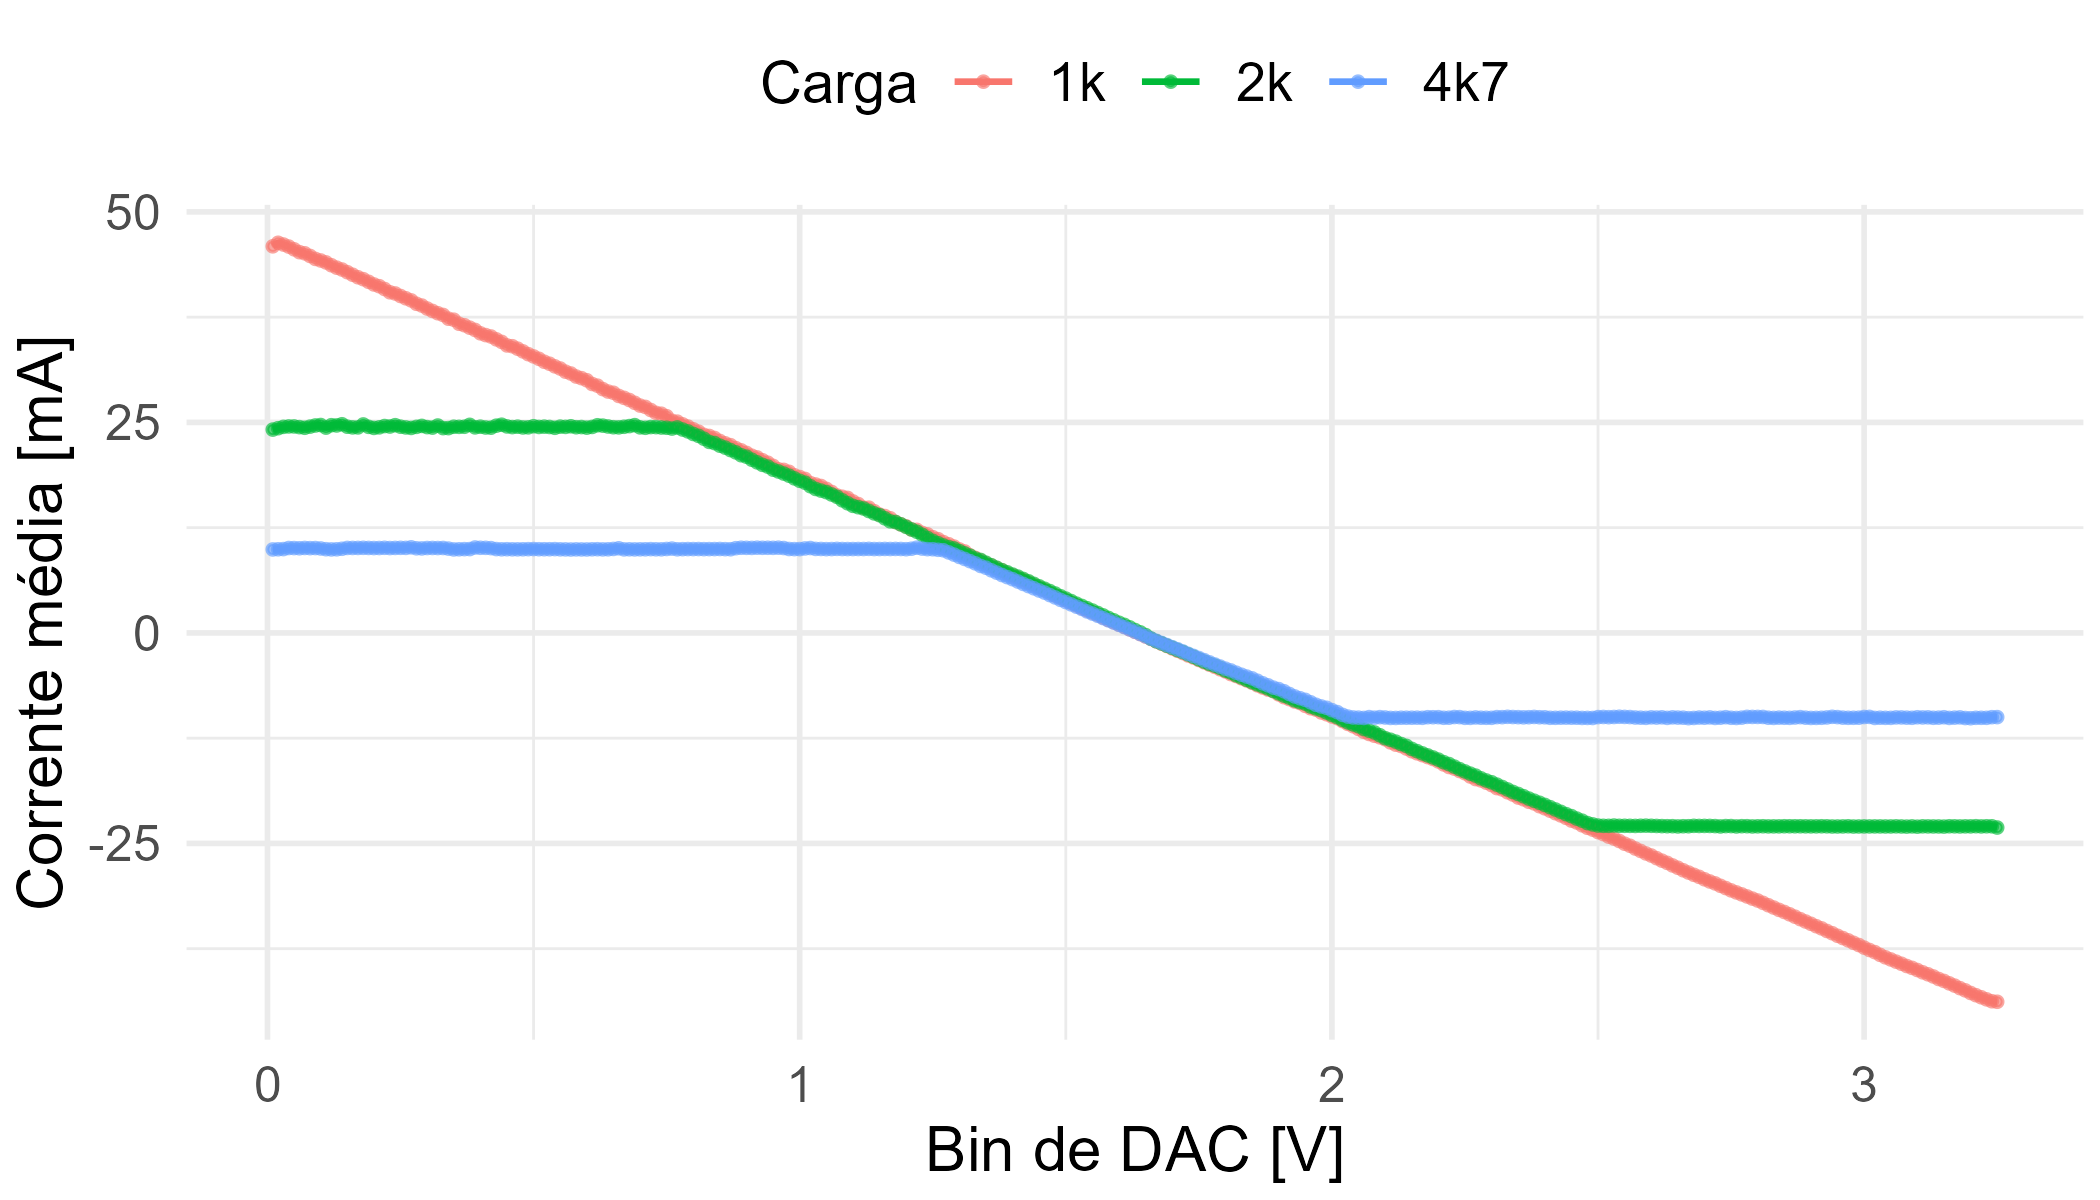
\includegraphics[width=0.78\linewidth,keepaspectratio]{figures/04_binned_current_by_load.png}
\captionof{figure}{Corrente média em função dos bins de DAC após a redução de granularidade}
\end{center}
\FloatBarrier

\FloatBarrier

\clearpage

\section{Identificação da região de
compliance}\label{identificauxe7uxe3o-da-regiuxe3o-de-compliance}

Em uma fonte de corrente, a região de compliance corresponde à faixa de
operação em que o circuito ainda possui tensão disponível suficiente
para impor a corrente comandada sobre a carga. Dentro dessa região, a
corrente depende predominantemente do comando aplicado ao estágio de
saída, e não da limitação de tensão dos componentes. Quando a carga exige
uma tensão maior do que a fonte consegue fornecer, o estágio se aproxima
da saturação: a corrente deixa de acompanhar linearmente o comando do DAC
e passam a aparecer desvios, oscilações e perda de previsibilidade.

A região comum de compliance foi definida antes da regressão usando dois
critérios: limite físico pela tensão reconstruída na carga e inclinação
local mínima compatível com o trecho linear de cada carga. O limite
comum de tensão foi tomado como a menor magnitude máxima de tensão
reconstruída entre as cargas, definindo uma faixa simétrica comum em
torno de zero; em seguida, foram mantidos apenas os pontos do maior
trecho contínuo com inclinação local suficiente. O modelo linear deve
ser interpretado apenas dentro dessa região comum.

\begin{center}
\scriptsize
\begin{tabular}{@{}llllll@{}}
\toprule
Carga & Faixa medida (V) & Faixa comum (V) & Pontos retidos & Pontos removidos & Removidos (\%) \\
\midrule
1k & -43.80 a 46.33 & -46.33 a 46.33 & 322 & 3 & 0.923 \\
2k & -46.22 a 49.56 & -46.33 a 46.33 & 168 & 157 & 48.308 \\
4k7 & -47.62 a 47.78 & -46.33 a 46.33 & 76 & 249 & 76.615 \\
\bottomrule
\end{tabular}
\end{center}
\tablecaptionbelow{Pontos retidos e removidos na identificação da região de compliance}

\begin{center}
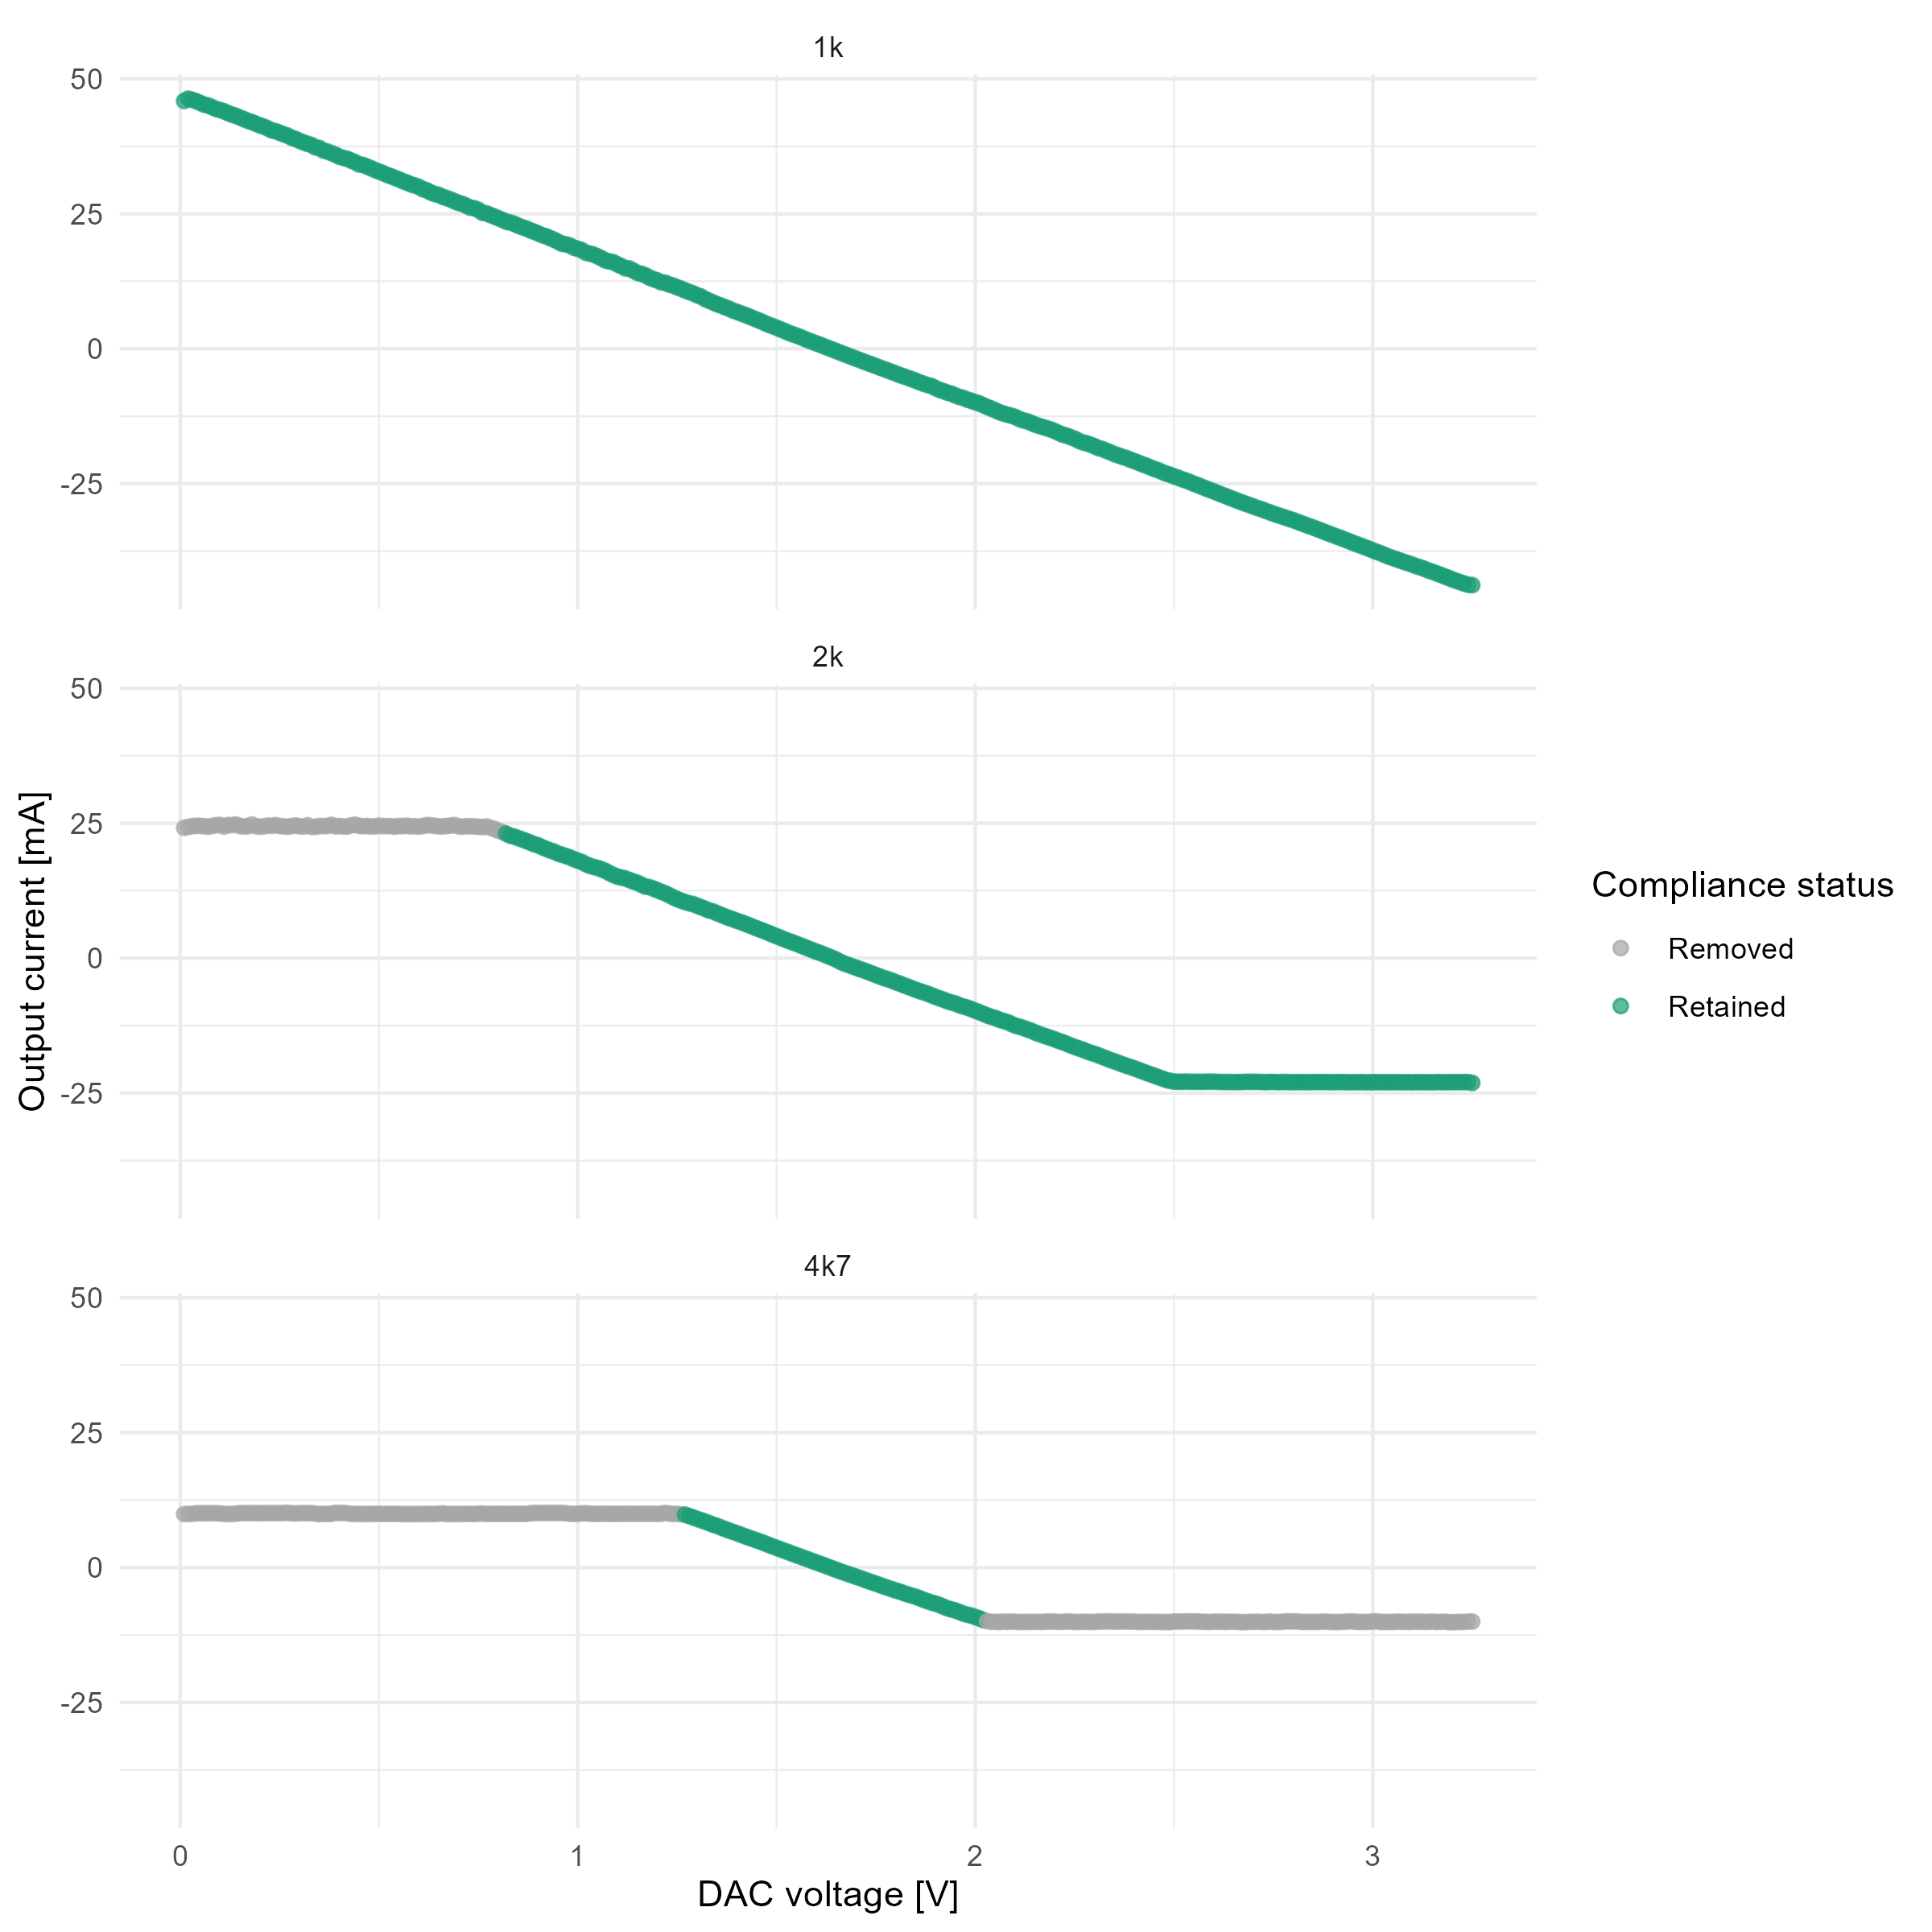
\includegraphics[width=0.72\linewidth,keepaspectratio]{figures/05_compliance_retained_removed.png}
\captionof{figure}{Pontos retidos e removidos pelo critério de compliance}
\end{center}
\FloatBarrier

\FloatBarrier

\newpage

\section{Estatística descritiva
relevante}\label{estatuxedstica-descritiva-relevante}

Resumo da região linear retida:

{\def\LTcaptype{none} % do not increment counter
\begin{longtable}[]{@{}
  >{\raggedright\arraybackslash}p{(\linewidth - 16\tabcolsep) * \real{0.1111}}
  >{\raggedright\arraybackslash}p{(\linewidth - 16\tabcolsep) * \real{0.1111}}
  >{\raggedright\arraybackslash}p{(\linewidth - 16\tabcolsep) * \real{0.1111}}
  >{\raggedright\arraybackslash}p{(\linewidth - 16\tabcolsep) * \real{0.1111}}
  >{\raggedright\arraybackslash}p{(\linewidth - 16\tabcolsep) * \real{0.1111}}
  >{\raggedright\arraybackslash}p{(\linewidth - 16\tabcolsep) * \real{0.1111}}
  >{\raggedright\arraybackslash}p{(\linewidth - 16\tabcolsep) * \real{0.1111}}
  >{\raggedright\arraybackslash}p{(\linewidth - 16\tabcolsep) * \real{0.1111}}
  >{\raggedright\arraybackslash}p{(\linewidth - 16\tabcolsep) * \real{0.1111}}@{}}
\toprule\noalign{}
\begin{minipage}[b]{\linewidth}\raggedright
Carga
\end{minipage} & \begin{minipage}[b]{\linewidth}\raggedright
N
\end{minipage} & \begin{minipage}[b]{\linewidth}\raggedright
Média (mA)
\end{minipage} & \begin{minipage}[b]{\linewidth}\raggedright
Desvio padrão (mA)
\end{minipage} & \begin{minipage}[b]{\linewidth}\raggedright
Mínimo (mA)
\end{minipage} & \begin{minipage}[b]{\linewidth}\raggedright
Q1 (mA)
\end{minipage} & \begin{minipage}[b]{\linewidth}\raggedright
Mediana (mA)
\end{minipage} & \begin{minipage}[b]{\linewidth}\raggedright
Q3 (mA)
\end{minipage} & \begin{minipage}[b]{\linewidth}\raggedright
Máximo (mA)
\end{minipage} \\
\midrule\noalign{}
\endhead
\bottomrule\noalign{}
\endlastfoot
1k & 322 & 0.645672 & 26.179311 & -43.739572 & -21.889446 & -0.004240 &
23.329117 & 46.122148 \\
2k & 168 & -0.142096 & 13.424850 & -22.740101 & -11.670383 & -0.463385 &
11.370625 & 23.062448 \\
4k7 & 76 & -0.107802 & 5.777173 & -9.731551 & -5.021909 & -0.269278 &
4.849080 & 9.812040 \\
\end{longtable}
}
\tablecaptionbelow{Resumo estatístico da região linear retida por carga}

\section{Correlação
exploratória}\label{correlauxe7uxe3o-exploratuxf3ria}

Correlação foi mantida apenas como evidência exploratória de associação
monotônica/linear entre DAC e corrente. A validade do circuito é
discutida a partir de erro, resíduos, intervalos e limites de
compliance.

{\def\LTcaptype{none} % do not increment counter
\begin{longtable}[]{@{}
  >{\raggedright\arraybackslash}p{(\linewidth - 10\tabcolsep) * \real{0.1667}}
  >{\raggedright\arraybackslash}p{(\linewidth - 10\tabcolsep) * \real{0.1667}}
  >{\raggedright\arraybackslash}p{(\linewidth - 10\tabcolsep) * \real{0.1667}}
  >{\raggedright\arraybackslash}p{(\linewidth - 10\tabcolsep) * \real{0.1667}}
  >{\raggedright\arraybackslash}p{(\linewidth - 10\tabcolsep) * \real{0.1667}}
  >{\raggedright\arraybackslash}p{(\linewidth - 10\tabcolsep) * \real{0.1667}}@{}}
\toprule\noalign{}
\begin{minipage}[b]{\linewidth}\raggedright
Carga
\end{minipage} & \begin{minipage}[b]{\linewidth}\raggedright
Correlação Pearson
\end{minipage} & \begin{minipage}[b]{\linewidth}\raggedright
Valor-p Pearson
\end{minipage} & \begin{minipage}[b]{\linewidth}\raggedright
Correlação Spearman
\end{minipage} & \begin{minipage}[b]{\linewidth}\raggedright
Valor-p Spearman
\end{minipage} & \begin{minipage}[b]{\linewidth}\raggedright
Amostras
\end{minipage} \\
\midrule\noalign{}
\endhead
\bottomrule\noalign{}
\endlastfoot
1k & -0.999909 & 0 & -1 & 0 & 322 \\
2k & -0.999897 & 0 & -1 & 0 & 168 \\
4k7 & -0.999815 & 0 & -1 & 0 & 76 \\
\end{longtable}
}
\tablecaptionbelow{Correlação exploratória entre tensão de DAC e corrente por carga}

\section{Modelos lineares por carga}\label{modelos-lineares-por-carga}

Para cada carga, foi ajustado um modelo linear independente relacionando
a corrente de saída ao nível de comando do DAC. Em termos estatísticos, o
modelo pode ser escrito como na Equação~\ref{eq:linear-model}:
\begin{equation}
I = \beta_0 + \beta_1 V_{\mathrm{DAC}} + \varepsilon,
\label{eq:linear-model}
\end{equation}
em que \(I\) é a corrente medida, \(V_{\mathrm{DAC}}\) é a tensão de DAC,
\(\beta_0\) é o coeficiente linear, \(\beta_1\) é o coeficiente angular e
\(\varepsilon\) representa o erro residual do ajuste.

{\def\LTcaptype{none} % do not increment counter
\begin{longtable}[]{@{}
  >{\raggedright\arraybackslash}p{(\linewidth - 16\tabcolsep) * \real{0.1111}}
  >{\raggedright\arraybackslash}p{(\linewidth - 16\tabcolsep) * \real{0.1111}}
  >{\raggedright\arraybackslash}p{(\linewidth - 16\tabcolsep) * \real{0.1111}}
  >{\raggedright\arraybackslash}p{(\linewidth - 16\tabcolsep) * \real{0.1111}}
  >{\raggedright\arraybackslash}p{(\linewidth - 16\tabcolsep) * \real{0.1111}}
  >{\raggedright\arraybackslash}p{(\linewidth - 16\tabcolsep) * \real{0.1111}}
  >{\raggedright\arraybackslash}p{(\linewidth - 16\tabcolsep) * \real{0.1111}}
  >{\raggedright\arraybackslash}p{(\linewidth - 16\tabcolsep) * \real{0.1111}}
  >{\raggedright\arraybackslash}p{(\linewidth - 16\tabcolsep) * \real{0.1111}}@{}}
\toprule\noalign{}
\begin{minipage}[b]{\linewidth}\raggedright
Modelo
\end{minipage} & \begin{minipage}[b]{\linewidth}\raggedright
Carga
\end{minipage} & \begin{minipage}[b]{\linewidth}\raggedright
R2
\end{minipage} & \begin{minipage}[b]{\linewidth}\raggedright
R2 ajustado
\end{minipage} & \begin{minipage}[b]{\linewidth}\raggedright
Desvio residual (mA)
\end{minipage} & \begin{minipage}[b]{\linewidth}\raggedright
Amostras
\end{minipage} & \begin{minipage}[b]{\linewidth}\raggedright
MAE (mA)
\end{minipage} & \begin{minipage}[b]{\linewidth}\raggedright
RMSE (mA)
\end{minipage} & \begin{minipage}[b]{\linewidth}\raggedright
Erro absoluto máximo (mA)
\end{minipage} \\
\midrule\noalign{}
\endhead
\bottomrule\noalign{}
\endlastfoot
Modelo da carga de 1 kOhm & 1k & 0.999818 & 0.999817 & 0.354077 & 322 & 0.287084 &
0.352975 & 0.743690 \\
Modelo da carga de 2 kOhm & 2k & 0.999794 & 0.999792 & 0.193410 & 168 & 0.159041 &
0.192255 & 0.445245 \\
Modelo da carga de 4,7 kOhm & 4k7 & 0.999630 & 0.999625 & 0.111824 & 76 & 0.095924 &
0.110343 & 0.252044 \\
\end{longtable}
}
\tablecaptionbelow{Desempenho dos modelos lineares independentes por carga}

As equações estimadas para cada carga estão reunidas na
Equação~\ref{eq:linear-models-by-load}:
\begin{equation}
\begin{aligned}
I_{1\,\mathrm{kOhm}}\,[\mathrm{mA}] &= 46{,}6181 - 28{,}1177\,V_{\mathrm{DAC}}\,[\mathrm{V}],\\
I_{2\,\mathrm{kOhm}}\,[\mathrm{mA}] &= 45{,}5305 - 27{,}5967\,V_{\mathrm{DAC}}\,[\mathrm{V}],\\
I_{4{,}7\,\mathrm{kOhm}}\,[\mathrm{mA}] &= 42{,}9190 - 26{,}1561\,V_{\mathrm{DAC}}\,[\mathrm{V}].
\end{aligned}
\label{eq:linear-models-by-load}
\end{equation}
Assim, os coeficientes angulares variam de aproximadamente -28,12 mA/V a
-26,16 mA/V, enquanto os coeficientes lineares variam de 46,62 mA a
42,92 mA. Essa diferença mostra que as retas por carga são muito
próximas, mas não exatamente coincidentes.

\newpage

\section{Modelo global}\label{modelo-global}

O modelo global foi ajustado dentro da região comum de compliance,
relacionando a corrente de saída ao nível de comando do DAC por uma única
reta, seguindo a mesma forma geral da Equação~\ref{eq:linear-model}:
\begin{equation}
I = \beta_0 + \beta_1 V_{\mathrm{DAC}} + \varepsilon.
\label{eq:global-model-general}
\end{equation}
Com os dados deste ensaio, a equação estimada foi a
Equação~\ref{eq:global-model-estimated}:
\begin{equation}
I\,[\mathrm{mA}] = 46{,}3489 - 28{,}0332\,V_{\mathrm{DAC}}\,[\mathrm{V}].
\label{eq:global-model-estimated}
\end{equation}
Assim, o coeficiente linear do modelo global é 46,3489 mA, e o
coeficiente angular é -28,0332 mA/V. O sinal negativo indica que, nesta
montagem, o aumento da tensão de DAC reduz a corrente calculada no
sentido adotado para o sinal.

Para obter esse modelo, não foi ajustada uma regressão separada para
cada carga. Após o binning e a seleção da região comum de compliance, os
dados das três cargas foram mantidos em formato longo em
\texttt{linear\_long}: cada linha contém um par (\texttt{dac\_bin},
\texttt{current\_mA}) e o rótulo da carga correspondente (\texttt{1k},
\texttt{2k} ou \texttt{4k7}). Em seguida, todas essas linhas foram
usadas juntas em uma única regressão linear.

Na prática, isso equivale a empilhar os pontos válidos das três cargas
em um único conjunto de observações. A identificação da carga permanece
disponível para gráficos e diagnósticos, mas não participa da equação do
modelo global. Assim, o ajuste estima uma única inclinação e um único
intercepto para representar a relação média entre comando de DAC e
corrente de saída, independentemente da carga, desde que os pontos
estejam dentro da região comum de compliance.

Esse procedimento é coerente com o objetivo de obter uma equação
operacional única para estimativa em malha aberta. Se as curvas das
cargas permanecem próximas após a remoção dos pontos limitados por
compliance, um único modelo global pode representar o comportamento do
estágio de saída sem exigir coeficientes específicos por carga. A
comparação posterior com o ajuste que inclui a influência da carga sobre
a relação DAC-corrente verifica justamente se adicionar dependência
explícita da carga melhora de forma relevante essa representação.

\begin{figure}
\centering
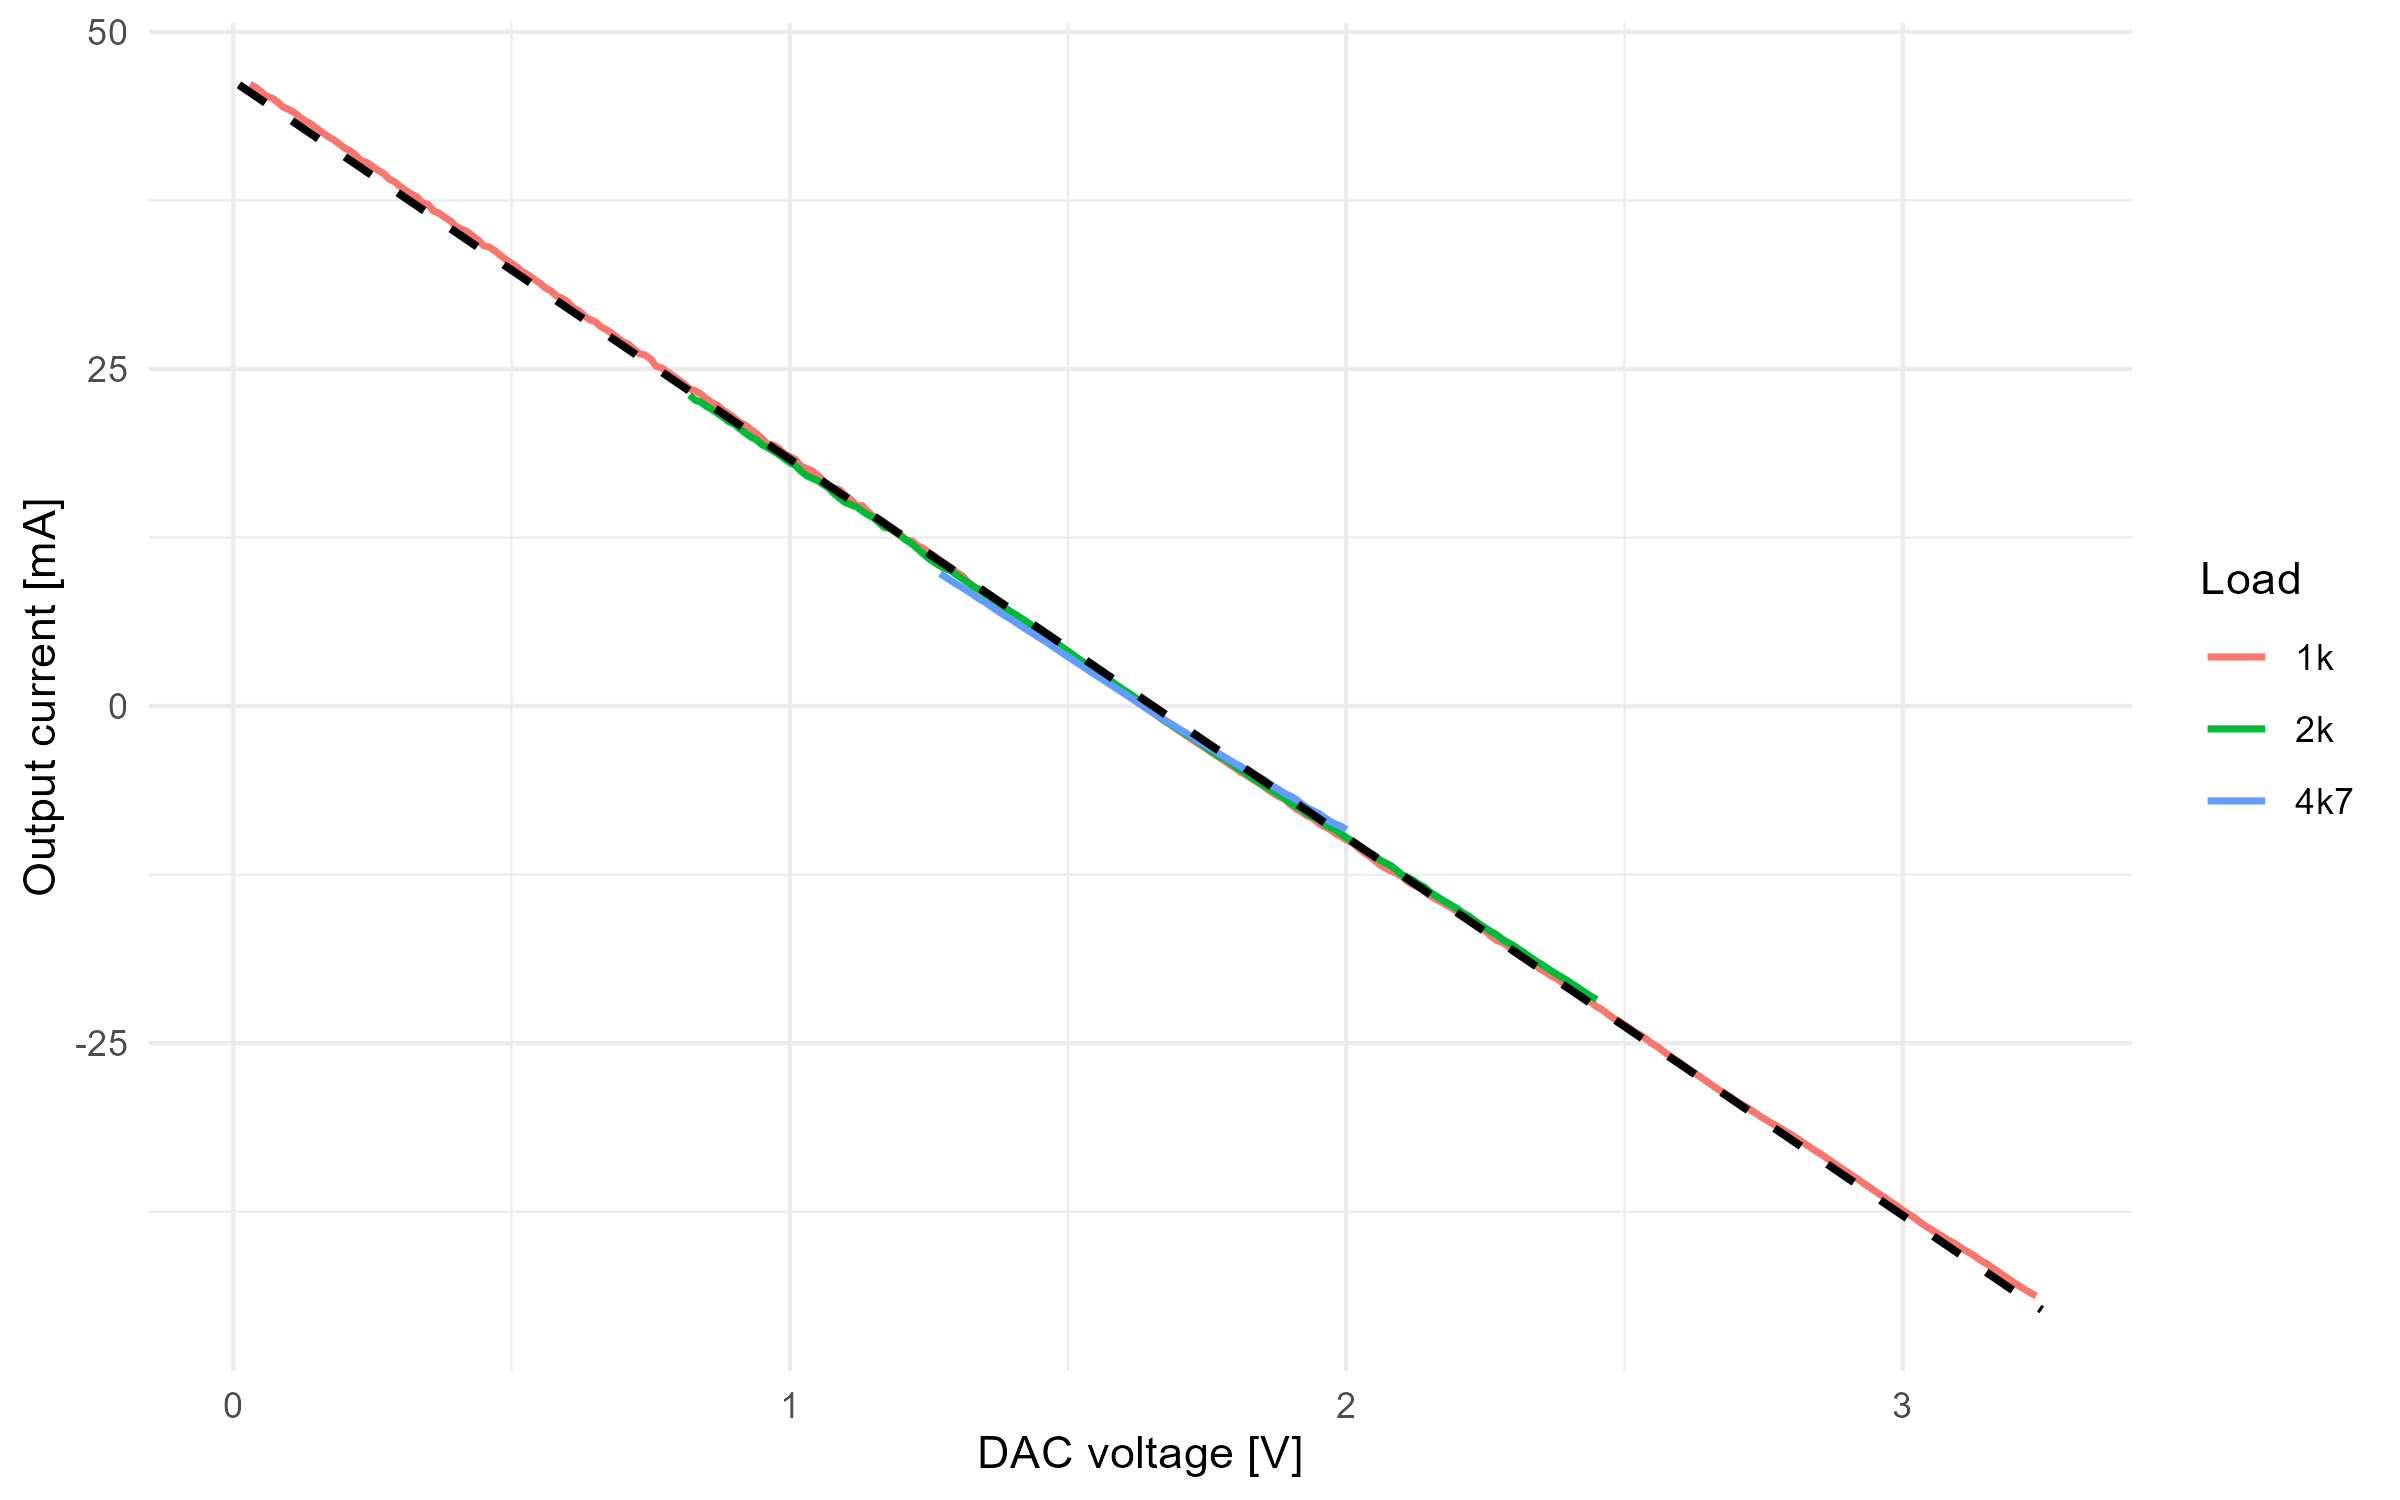
\includegraphics[width=0.92\linewidth,keepaspectratio]{figures/06_linear_region_global_model.png}
\caption{Curvas experimentais de corrente e modelo linear global}
\end{figure}

\FloatBarrier

A figura permite avaliar visualmente o compromisso do modelo global: a
reta única acompanha bem a tendência média das três cargas, mas pequenos
desvios sistemáticos entre as cores indicam que as curvas não são
perfeitamente coincidentes. Essa diferença visual antecipa a análise da
influência da carga sobre a relação DAC-corrente, que testa formalmente
se a carga altera a relação entre DAC e corrente.

{\def\LTcaptype{none} % do not increment counter
\begin{longtable}[]{@{}
  >{\raggedright\arraybackslash}p{(\linewidth - 14\tabcolsep) * \real{0.1250}}
  >{\raggedright\arraybackslash}p{(\linewidth - 14\tabcolsep) * \real{0.1250}}
  >{\raggedright\arraybackslash}p{(\linewidth - 14\tabcolsep) * \real{0.1250}}
  >{\raggedright\arraybackslash}p{(\linewidth - 14\tabcolsep) * \real{0.1250}}
  >{\raggedright\arraybackslash}p{(\linewidth - 14\tabcolsep) * \real{0.1250}}
  >{\raggedright\arraybackslash}p{(\linewidth - 14\tabcolsep) * \real{0.1250}}
  >{\raggedright\arraybackslash}p{(\linewidth - 14\tabcolsep) * \real{0.1250}}
  >{\raggedright\arraybackslash}p{(\linewidth - 14\tabcolsep) * \real{0.1250}}@{}}
\toprule\noalign{}
\begin{minipage}[b]{\linewidth}\raggedright
\textbf{Modelo}
\end{minipage} & \begin{minipage}[b]{\linewidth}\raggedright
\textbf{R2}
\end{minipage} & \begin{minipage}[b]{\linewidth}\raggedright
\textbf{R2 ajustado}
\end{minipage} & \begin{minipage}[b]{\linewidth}\raggedright
\textbf{Desvio residual (mA)}
\end{minipage} & \begin{minipage}[b]{\linewidth}\raggedright
\textbf{Amostras}
\end{minipage} & \begin{minipage}[b]{\linewidth}\raggedright
\textbf{MAE (mA)}
\end{minipage} & \begin{minipage}[b]{\linewidth}\raggedright
\textbf{RMSE (mA)}
\end{minipage} & \begin{minipage}[b]{\linewidth}\raggedright
\textbf{Erro absoluto máximo (mA)}
\end{minipage} \\
\midrule\noalign{}
\endhead
\bottomrule\noalign{}
\endlastfoot
Modelo global & 0.999661 & 0.999661 & 0.389648 & 566 &
0.331486 & 0.388959 & 0.934792 \\
\end{longtable}
}
\tablecaptionbelow{Desempenho do modelo global para a região linear retida}

\section{Influência da carga sobre a relação DAC-corrente}
\label{modelo-com-influencia-carga-dac}

Este tópico usa uma extensão direta da regressão linear múltipla
apresentada na disciplina. A tensão de DAC é tratada como variável
explicativa quantitativa, enquanto a carga resistiva é tratada como
variável categórica. Como modelos de regressão não utilizam diretamente
nomes de categorias, as cargas são representadas por variáveis
indicadoras, também chamadas de variáveis \emph{dummies}. Neste relatório,
essas variáveis são indicadas pela letra \(D\), justamente para
diferenciá-las da resistência física da carga. Elas permitem incluir no
mesmo modelo o fato de a medição pertencer à carga de 1 kOhm, 2 kOhm ou
4,7 kOhm.

No modelo global, uma única reta é usada para representar todas
as cargas, assumindo o mesmo intercepto e a mesma inclinação. Essa
hipótese é simples e útil, mas pode esconder pequenas diferenças entre as
cargas. Ao incluir a influência da carga sobre a relação DAC-corrente,
verifica-se se a relação entre tensão de DAC e corrente é a mesma para
todas as cargas ou se muda levemente conforme a carga conectada.

Em termos estatísticos, essa influência é representada por termos que
permitem que o efeito de uma variável explicativa dependa da carga
conectada. Neste relatório, isso significa perguntar se a variação da
corrente causada por uma mudança na tensão de DAC é igual para todas as
cargas. Se a influência da carga for pequena, as retas associadas às
cargas tendem a ser aproximadamente paralelas. Se ela for relevante, a
inclinação da reta também muda com a carga. Assim, a carga pode alterar
tanto o deslocamento vertical da reta quanto sua inclinação, conforme a
Equação~\ref{eq:influence-model-general}:
\begin{equation}
I = \beta_0 + \beta_1 V_{\mathrm{DAC}} + \gamma_R +
\delta_R V_{\mathrm{DAC}} + \varepsilon,
\label{eq:influence-model-general}
\end{equation}
em que \(I\) é a corrente medida e \(V_{\mathrm{DAC}}\) é a tensão de
comando do DAC. Essa forma resume a ideia geral do modelo: a carga de
referência possui uma reta própria, e as demais cargas entram como
correções dessa reta. Os parâmetros são:

\begin{itemize}
\tightlist
\item
  \(\beta_0\): intercepto da carga de referência, neste caso 1 kOhm;
\item
  \(\beta_1\): inclinação da reta da carga de referência;
\item
  \(\gamma_R\): deslocamento vertical da reta para outra carga \(R\);
\item
  \(\delta_R\): alteração da inclinação da reta para outra carga \(R\);
\item
  \(\varepsilon\): erro residual, isto é, a diferença não explicada pelo
  modelo.
\end{itemize}

Neste ajuste, portanto, a carga de 1 kOhm é tomada como referência. Essa
escolha não significa que ela seja mais importante fisicamente; trata-se
apenas de uma convenção estatística para escrever o modelo sem
redundância. Como existem três cargas, são necessárias apenas duas
variáveis indicadoras: \(D_{2k}\) para a carga de 2 kOhm e
\(D_{4{,}7k}\) para a carga de 4,7 kOhm. Quando ambas valem zero, a
observação pertence automaticamente à carga de 1 kOhm.

Esse procedimento evita multicolinearidade perfeita. Se fossem usadas
três variáveis indicadoras, uma para cada carga, junto com o intercepto do
modelo, haveria uma relação linear exata entre elas, pois a soma das três
indicadoras seria sempre igual a 1. Nesse caso, uma coluna da matriz de
regressão poderia ser escrita como combinação das demais, e os
coeficientes não seriam estimados de forma única. Ao omitir a dummy da
carga de referência, o modelo mantém a mesma informação categórica sem
criar essa redundância. Os termos associados a 2 kOhm e 4,7 kOhm indicam
quanto essas cargas se afastam da reta de referência.

Em termos simples, essa formulação testa se mudar a carga apenas desloca
a curva para cima ou para baixo, ou se também modifica a sensibilidade da
corrente ao comando de DAC. Se os termos produto entre DAC e carga forem
relevantes, isso indica que as curvas das cargas não são paralelas: além
de terem interceptos diferentes, também possuem inclinações ligeiramente
distintas.

A equação completa estimada para o ajuste com influência da carga é dada
pela Equação~\ref{eq:influence-model-estimated}:
\begin{equation}
\begin{aligned}
I\,[\mathrm{mA}] =\;& 46{,}6181
- 28{,}1177\,V_{\mathrm{DAC}}\,[\mathrm{V}]
- 1{,}0877\,D_{2k}
- 3{,}6991\,D_{4{,}7k}\\
&+ 0{,}5210\,V_{\mathrm{DAC}}\,[\mathrm{V}]\,D_{2k}
+ 1{,}9616\,V_{\mathrm{DAC}}\,[\mathrm{V}]\,D_{4{,}7k},
\end{aligned}
\label{eq:influence-model-estimated}
\end{equation}
em que \(D_{2k}\) é uma variável indicadora que vale 1 quando a carga
resistiva é 2 kOhm e 0 nos demais casos, e \(D_{4{,}7k}\) é uma variável
indicadora que vale 1 quando a carga resistiva é 4,7 kOhm e 0 nos demais
casos. Para a carga de 1 kOhm, ambas as variáveis indicadoras valem 0,
pois ela é a referência do modelo. Aqui, \(D_{2k}\) e \(D_{4{,}7k}\) não
representam valores de resistência em ohms, mas apenas a presença de cada
carga no ajuste.

A partir dos coeficientes do ajuste com influência da carga, as retas
finais por carga são obtidas conforme a Equação~\ref{eq:influence-lines}:
\begin{equation}
\begin{aligned}
I_{1\,\mathrm{kOhm}}\,[\mathrm{mA}] &= 46{,}6181 - 28{,}1177\,V_{\mathrm{DAC}}\,[\mathrm{V}]\\[1.0em]
I_{2\,\mathrm{kOhm}}\,[\mathrm{mA}] &= (46{,}6181 - 1{,}0877) + (-28{,}1177 + 0{,}5210)\,V_{\mathrm{DAC}}\,[\mathrm{V}]
= 45{,}5305 - 27{,}5967\,V_{\mathrm{DAC}}\,[\mathrm{V}]\\[1.0em]
I_{4{,}7\,\mathrm{kOhm}}\,[\mathrm{mA}] &= (46{,}6181 - 3{,}6991) + (-28{,}1177 + 1{,}9616)\,V_{\mathrm{DAC}}\,[\mathrm{V}]
= 42{,}9190 - 26{,}1561\,V_{\mathrm{DAC}}\,[\mathrm{V}].
\end{aligned}
\label{eq:influence-lines}
\end{equation}

Essas equações deixam explícito que o ajuste com influência da carga não
produz uma única reta igual à do modelo global. Ele produz uma reta de
referência para 1 kOhm e aplica correções de intercepto e inclinação para
2 kOhm e 4,7 kOhm.

\begin{figure}
\centering
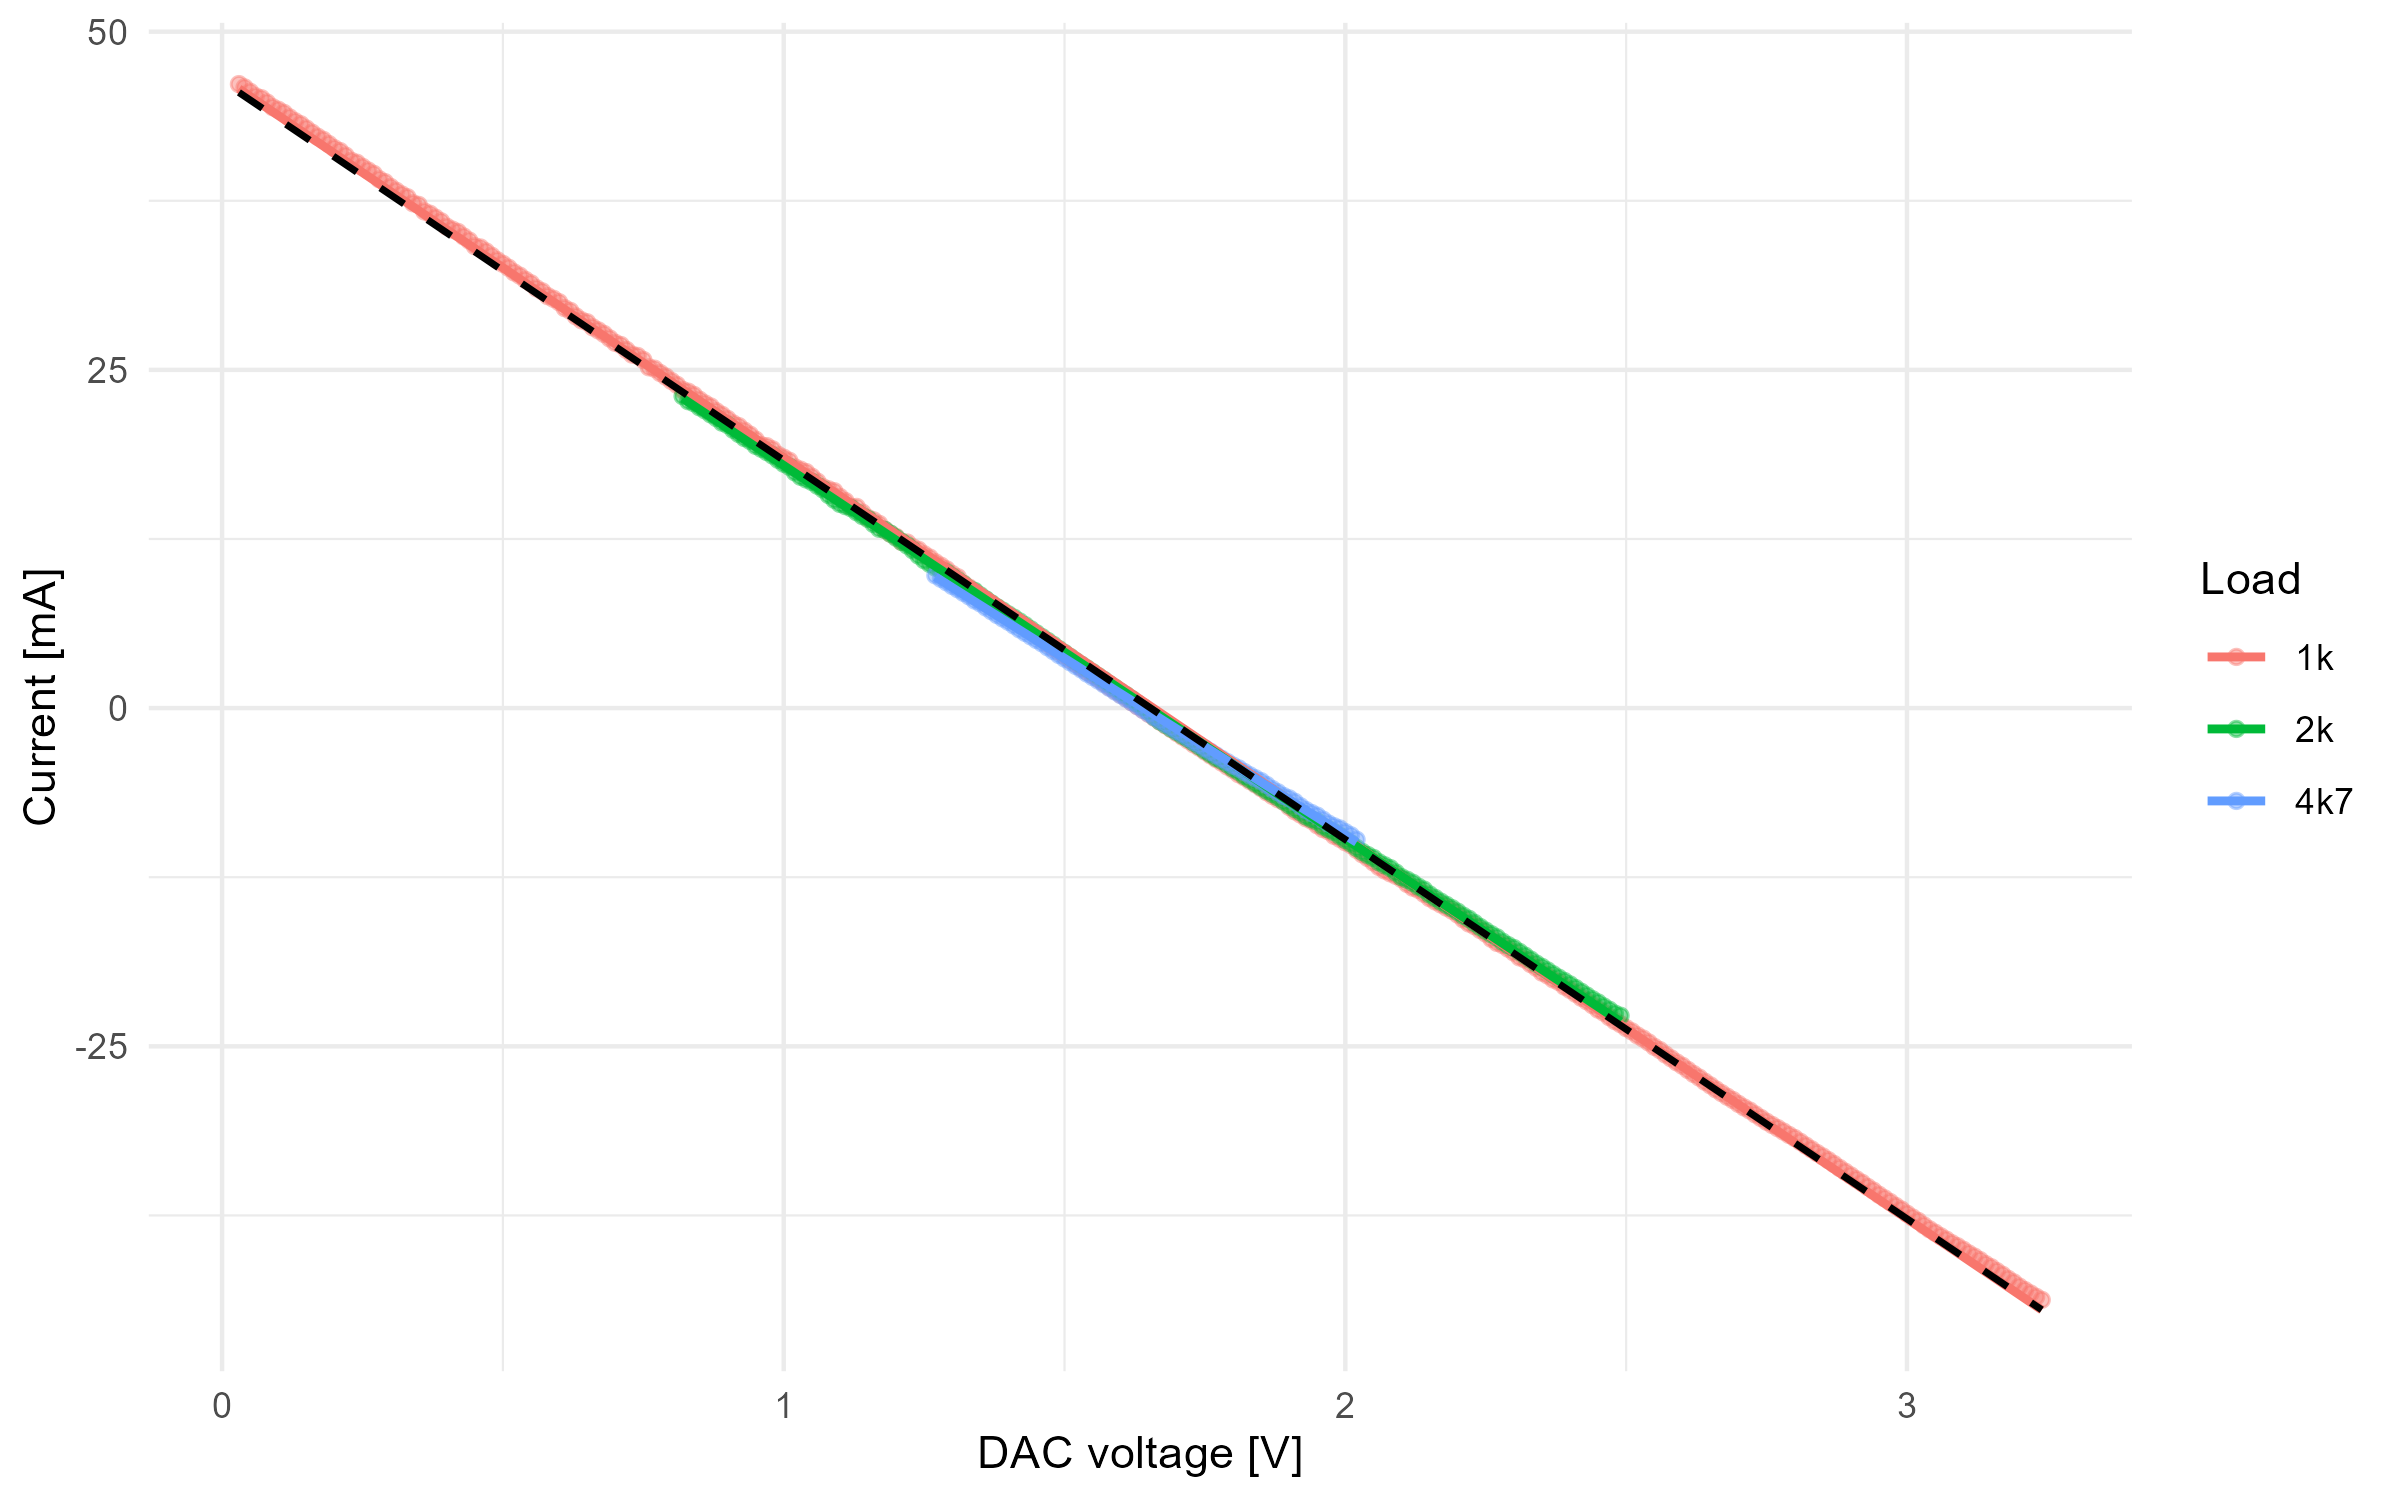
\includegraphics[width=0.92\linewidth,keepaspectratio]{figures/07_interaction_model_by_load.png}
\caption{Retas estimadas pelo ajuste com influência da carga sobre a relação DAC-corrente}
\end{figure}

\FloatBarrier

A figura mostra a diferença prática entre o modelo global e o ajuste com
influência da carga. A linha preta tracejada representa a reta global única,
enquanto as linhas coloridas representam as retas estimadas para cada
carga dentro de uma mesma formulação estatística. A proximidade entre as
retas confirma que o comportamento geral é muito semelhante, mas a
separação entre elas mostra por que a inclusão da carga reduz o erro
residual.

As métricas de desempenho resumem o ajuste completo com influência da carga. Embora
o modelo contenha termos específicos para as cargas de 2 kOhm e 4,7 kOhm
em relação à referência de 1 kOhm, ele constitui uma única formulação
estatística e, por isso, é apresentado como um único ajuste.

{\def\LTcaptype{none} % do not increment counter
\begin{longtable}[]{@{}
  >{\raggedright\arraybackslash}p{(\linewidth - 14\tabcolsep) * \real{0.1250}}
  >{\raggedright\arraybackslash}p{(\linewidth - 14\tabcolsep) * \real{0.1250}}
  >{\raggedright\arraybackslash}p{(\linewidth - 14\tabcolsep) * \real{0.1250}}
  >{\raggedright\arraybackslash}p{(\linewidth - 14\tabcolsep) * \real{0.1250}}
  >{\raggedright\arraybackslash}p{(\linewidth - 14\tabcolsep) * \real{0.1250}}
  >{\raggedright\arraybackslash}p{(\linewidth - 14\tabcolsep) * \real{0.1250}}
  >{\raggedright\arraybackslash}p{(\linewidth - 14\tabcolsep) * \real{0.1250}}
  >{\raggedright\arraybackslash}p{(\linewidth - 14\tabcolsep) * \real{0.1250}}@{}}
\toprule\noalign{}
\begin{minipage}[b]{\linewidth}\raggedright
\textbf{Modelo}
\end{minipage} & \begin{minipage}[b]{\linewidth}\raggedright
\textbf{R2}
\end{minipage} & \begin{minipage}[b]{\linewidth}\raggedright
\textbf{R2 ajustado}
\end{minipage} & \begin{minipage}[b]{\linewidth}\raggedright
\textbf{Desvio residual (mA)}
\end{minipage} & \begin{minipage}[b]{\linewidth}\raggedright
\textbf{Amostras}
\end{minipage} & \begin{minipage}[b]{\linewidth}\raggedright
\textbf{MAE (mA)}
\end{minipage} & \begin{minipage}[b]{\linewidth}\raggedright
\textbf{RMSE (mA)}
\end{minipage} & \begin{minipage}[b]{\linewidth}\raggedright
\textbf{Erro absoluto máximo (mA)}
\end{minipage} \\
\midrule\noalign{}
\endhead
\bottomrule\noalign{}
\endlastfoot
Influência carga-DAC & 0.999813 & 0.999811 & 0.290484
& 566 & 0.223411 & 0.288941 & 0.74369 \\
\end{longtable}
}
\tablecaptionbelow{Desempenho do ajuste com influência da carga sobre a relação DAC-corrente}

Ao incluir a influência da carga sobre a relação DAC-corrente, o ajuste reduz o
desvio residual, o MAE, o RMSE e o erro absoluto máximo em relação ao
modelo global. Em termos práticos, isso indica que as curvas das três
cargas são muito próximas, mas não perfeitamente coincidentes. A carga
não afeta apenas um deslocamento fixo da curva: ela também altera
levemente a inclinação da relação DAC-corrente. Portanto, para descrição
estatística dos dados, o ajuste com influência da carga representa melhor o
comportamento observado. Para uma aplicação embarcada simples em malha
aberta, porém, o modelo global ainda pode ser preferível se o erro
adicional for aceitável, pois o uso dessa influência exige conhecer ou
estimar a carga conectada para aplicar os coeficientes corretos.

Nas tabelas de coeficientes, \(H_0\) representa a hipótese nula de que o
coeficiente avaliado é igual a zero. Com nível de significância de 5\%
(\(\alpha = 0{,}05\)), a decisão ``rejeita \(H_0\)'' significa que o
p-valor ficou abaixo de 0,05 e há evidência estatística de que aquele
termo contribui para o modelo. A decisão ``não rejeita \(H_0\)''
significa que o teste não encontrou evidência suficiente, nesse nível de
significância, para afirmar que o coeficiente seja diferente de zero.
Isso não prova que o coeficiente seja exatamente zero; apenas indica
ausência de evidência estatística suficiente contra \(H_0\).

A tabela de coeficientes identifica, na coluna Modelo, a formulação de
regressão de onde cada estimativa foi obtida. A coluna Termo indica o
parâmetro avaliado, como intercepto, inclinação associada ao nível de DAC
ou efeitos adicionais de carga e dos termos produto DAC-carga. A Estimativa é o valor
calculado para o coeficiente, enquanto o Erro padrão representa a
incerteza dessa estimativa. A Estatística corresponde à razão entre a
estimativa e seu erro padrão, sendo usada no teste de significância do
coeficiente. O Valor-p quantifica a evidência contra \(H_0\), e o IC
95\% apresenta o intervalo de confiança de 95\% para o valor do
coeficiente.

{\def\LTcaptype{none} % do not increment counter
\begin{longtable}[]{@{}
  >{\raggedright\arraybackslash}p{(\linewidth - 12\tabcolsep) * \real{0.1700}}
  >{\raggedright\arraybackslash}p{(\linewidth - 12\tabcolsep) * \real{0.2200}}
  >{\raggedright\arraybackslash}p{(\linewidth - 12\tabcolsep) * \real{0.1000}}
  >{\raggedright\arraybackslash}p{(\linewidth - 12\tabcolsep) * \real{0.1000}}
  >{\raggedright\arraybackslash}p{(\linewidth - 12\tabcolsep) * \real{0.1200}}
  >{\raggedright\arraybackslash}p{(\linewidth - 12\tabcolsep) * \real{0.0800}}
  >{\raggedright\arraybackslash}p{(\linewidth - 12\tabcolsep) * \real{0.2100}}@{}}
\toprule\noalign{}
\begin{minipage}[b]{\linewidth}\raggedright
\textbf{Modelo}
\end{minipage} & \begin{minipage}[b]{\linewidth}\raggedright
\textbf{Termo}
\end{minipage} & \begin{minipage}[b]{\linewidth}\raggedright
\textbf{Estimativa}
\end{minipage} & \begin{minipage}[b]{\linewidth}\raggedright
\textbf{Erro padrão}
\end{minipage} & \begin{minipage}[b]{\linewidth}\raggedright
\textbf{Estatística}
\end{minipage} & \begin{minipage}[b]{\linewidth}\raggedright
\textbf{Valor-p}
\end{minipage} & \begin{minipage}[b]{\linewidth}\raggedright
\textbf{IC 95\%}
\end{minipage} \\
\midrule\noalign{}
\endhead
\bottomrule\noalign{}
\endlastfoot
Modelo global & Intercepto & 46,3489 & 0,0393 & 1180,24 &
\(<0{,}001\) & [46,2718; 46,4261] \\
\midrule
Modelo global & Nível de DAC & -28,0332 & 0,0217 & -1289,86 &
\(<0{,}001\) & [-28,0758; -27,9905] \\
\midrule
Influência carga-DAC & Intercepto & 46,6181 & 0,0328 & 1423,28 &
\(<0{,}001\) & [46,5538; 46,6825] \\
\midrule
Influência carga-DAC & Nível de DAC & -28,1177 & 0,0174 & -1614,54 &
\(<0{,}001\) & [-28,1519; -28,0835] \\
\midrule
Influência carga-DAC & Carga de 2 kOhm & -1,0877 & 0,0862 & -12,62 &
\(<0{,}001\) & [-1,2569; -0,9184] \\
\midrule
Influência carga-DAC & Carga de 4,7 kOhm & -3,6991 & 0,2542 & -14,55 &
\(<0{,}001\) & [-4,1984; -3,1998] \\
\midrule
Influência carga-DAC & Produto DAC-carga de 2 kOhm & 0,5210 & 0,0494 & 10,55 &
\(<0{,}001\) & [0,4240; 0,6180] \\
\midrule
Influência carga-DAC & Produto DAC-carga de 4,7 kOhm & 1,9616 & 0,1529 & 12,83 &
\(<0{,}001\) & [1,6613; 2,2619] \\
\midrule
Modelo da carga de 1 kOhm & Intercepto & 46,6181 & 0,0399 & 1167,66 &
\(<0{,}001\) & [46,5396; 46,6967] \\
\midrule
Modelo da carga de 1 kOhm & Nível de DAC & -28,1177 & 0,0212 & -1324,57 &
\(<0{,}001\) & [-28,1595; -28,0760] \\
\midrule
Modelo da carga de 2 kOhm & Intercepto & 45,5305 & 0,0531 & 858,03 &
\(<0{,}001\) & [45,4257; 45,6352] \\
\midrule
Modelo da carga de 2 kOhm & Nível de DAC & -27,5967 & 0,0308 & -896,90 &
\(<0{,}001\) & [-27,6575; -27,5360] \\
\midrule
Modelo da carga de 4,7 kOhm & Intercepto & 42,9190 & 0,0970 & 442,30 &
\(<0{,}001\) & [42,7257; 43,1124] \\
\midrule
Modelo da carga de 4,7 kOhm & Nível de DAC & -26,1561 & 0,0585 & -447,33 &
\(<0{,}001\) & [-26,2726; -26,0396] \\
\end{longtable}
}
\tablecaptionbelow{Coeficientes estimados e testes de significância dos modelos lineares}

Todos os coeficientes listados apresentam p-valor inferior a 0,001.
Portanto, para o nível de significância adotado de 5\%, todos levam à
rejeição de \(H_0\), indicando evidência estatística de contribuição dos
respectivos termos aos modelos.

\section{Comparação entre modelos}\label{comparauxe7uxe3o-entre-modelos}

A comparação formal entre o modelo global e o ajuste com influência da
carga sobre a relação DAC-corrente foi feita por ANOVA/teste F para modelos
aninhados.

Nessa comparação, o modelo global é o modelo reduzido, pois usa uma única
reta média para todas as cargas. O ajuste com influência da carga é o modelo
completo, pois adiciona termos para representar diferenças de intercepto e
inclinação entre as cargas. A comparação avalia se a redução do erro
residual obtida pelo modelo completo é grande o suficiente para justificar
os parâmetros adicionais.

O teste F é adequado nesse caso porque os modelos são aninhados: o modelo
global pode ser visto como uma versão simplificada do modelo com influência
da carga, obtida quando os termos adicionais de carga e os termos produto
DAC-carga são considerados
nulos. Assim, a hipótese nula do teste é apresentada na
Equação~\ref{eq:anova-h0}:
\begin{equation}
\begin{aligned}
H_0 &: \text{os termos adicionais de carga e produto DAC-carga}\\
&\quad \text{não reduzem o erro de forma relevante}.
\end{aligned}
\label{eq:anova-h0}
\end{equation}
A hipótese alternativa é apresentada na Equação~\ref{eq:anova-h1}:
\begin{equation}
\begin{aligned}
H_1 &: \text{os termos adicionais reduzem o erro residual}\\
&\quad \text{de forma estatisticamente significativa}.
\end{aligned}
\label{eq:anova-h1}
\end{equation}
Portanto, o teste não verifica se o modelo completo é ``perfeito'', mas
se ele melhora o ajuste em relação ao modelo mais simples.

A quantidade central da comparação é a soma dos quadrados residual,
definida pela Equação~\ref{eq:sq-residual}:
\begin{equation}
SQ_{\mathrm{res}} = \sum_{i=1}^{n} (I_i - \hat{I}_i)^2,
\label{eq:sq-residual}
\end{equation}
em que \(I_i\) é a corrente medida na \(i\)-ésima observação e
\(\hat{I}_i\) é a corrente prevista pelo modelo para essa mesma
observação. Portanto, quanto menor \(SQ_{\mathrm{res}}\), menor é a
variabilidade dos dados que permanece não explicada pelo modelo.

A estatística F compara duas quantidades: no numerador, a redução média do
erro residual obtida ao adicionar os novos parâmetros; no denominador, o
erro residual médio que ainda permanece no modelo completo. Para dois
modelos aninhados, essa razão pode ser escrita conforme a
Equação~\ref{eq:f-test}:
\begin{equation}
F =
\frac{(SQ_{\mathrm{res,red}} - SQ_{\mathrm{res,comp}})/(gl_{\mathrm{red}} - gl_{\mathrm{comp}})}
{SQ_{\mathrm{res,comp}}/gl_{\mathrm{comp}}},
\label{eq:f-test}
\end{equation}
em que \(SQ_{\mathrm{res,red}}\) é a soma dos quadrados residual do modelo
reduzido, \(SQ_{\mathrm{res,comp}}\) é a soma dos quadrados residual do
modelo completo, e \(gl\) representa os graus de liberdade residuais. Um
valor de F próximo de 1 indicaria que a melhoria obtida pelo modelo mais
complexo é pequena em relação ao erro que ainda sobra. Valores muito
maiores que 1 indicam que a melhoria é grande quando comparada à
variabilidade residual remanescente.

{\def\LTcaptype{none} % do not increment counter
\begin{longtable}[]{@{}
  >{\raggedright\arraybackslash}p{(\linewidth - 14\tabcolsep) * \real{0.1250}}
  >{\raggedright\arraybackslash}p{(\linewidth - 14\tabcolsep) * \real{0.1250}}
  >{\raggedright\arraybackslash}p{(\linewidth - 14\tabcolsep) * \real{0.1250}}
  >{\raggedright\arraybackslash}p{(\linewidth - 14\tabcolsep) * \real{0.1250}}
  >{\raggedright\arraybackslash}p{(\linewidth - 14\tabcolsep) * \real{0.1250}}
  >{\raggedright\arraybackslash}p{(\linewidth - 14\tabcolsep) * \real{0.1250}}
  >{\raggedright\arraybackslash}p{(\linewidth - 14\tabcolsep) * \real{0.1250}}
  >{\raggedright\arraybackslash}p{(\linewidth - 14\tabcolsep) * \real{0.1250}}@{}}
\toprule\noalign{}
\begin{minipage}[b]{\linewidth}\raggedright
\textbf{Modelo}
\end{minipage} & \begin{minipage}[b]{\linewidth}\raggedright
\textbf{Índice do modelo}
\end{minipage} & \begin{minipage}[b]{\linewidth}\raggedright
\textbf{GL residual}
\end{minipage} & \begin{minipage}[b]{\linewidth}\raggedright
\textbf{Soma quad. residual}
\end{minipage} & \begin{minipage}[b]{\linewidth}\raggedright
\textbf{GL}
\end{minipage} & \begin{minipage}[b]{\linewidth}\raggedright
\textbf{Soma dos quadrados}
\end{minipage} & \begin{minipage}[b]{\linewidth}\raggedright
\textbf{Estatística F}
\end{minipage} & \begin{minipage}[b]{\linewidth}\raggedright
\textbf{Valor-p (F)}
\end{minipage} \\
\midrule\noalign{}
\endhead
\bottomrule\noalign{}
\endlastfoot
Modelo global & 1 & 564 & 85.629792 & & & & \\
\midrule
Influência carga-DAC & 2 & 560 &
47.253472 & 4 & 38.37632 & 113.699262 & \(<0{,}001\) \\
\end{longtable}
}
\tablecaptionbelow{Comparação por ANOVA entre o modelo global e o ajuste com influência da carga}

Na tabela, o valor 85,63 mA\textsuperscript{2} corresponde ao
\(SQ_{\mathrm{res}}\) do modelo global, enquanto 47,25
mA\textsuperscript{2} corresponde ao \(SQ_{\mathrm{res}}\) do ajuste com
influência da carga. A diferença entre esses valores é dada pela
Equação~\ref{eq:sq-residual-reduction}:
\begin{equation}
85{,}63 - 47{,}25 = 38{,}38\ \mathrm{mA}^2,
\label{eq:sq-residual-reduction}
\end{equation}
que representa a redução da soma dos quadrados residual ao adicionar os
termos de carga e produto DAC-carga. O modelo completo usa quatro parâmetros
adicionais em relação ao modelo global, por isso a coluna GL da segunda
linha mostra o valor 4. Substituindo os valores na expressão do teste da
Equação~\ref{eq:f-test}, obtém-se:
\begin{equation}
F =
\frac{(85{,}629792 - 47{,}253472)/4}
{47{,}253472/560}
= 113{,}699262.
\label{eq:f-test-value}
\end{equation}
Esse número significa que a redução média do erro obtida pelos termos
adicionais é cerca de 113,7 vezes maior que o erro residual médio que
ainda permanece no modelo completo. Trata-se de uma razão muito alta, o
que indica que a melhora não é pequena em relação à variabilidade
remanescente.

O valor-p associado à estatística F é inferior a 0,001. Portanto, para o
nível de significância de 5\%, rejeita-se \(H_0\). Em termos práticos, há
evidência estatística de que considerar a influência da carga sobre a
relação DAC-corrente melhora o ajuste em relação ao modelo global. Assim, para
fins de descrição estatística dos dados experimentais, a formulação com
influência da carga é superior; para controle simples em malha aberta, o modelo
global ainda pode ser útil se o erro adicional for aceitável.

\section{Erro de predição}\label{erro-de-prediuxe7uxe3o}

As métricas de erro foram calculadas dentro da região linear: MAE, RMSE
e maior erro absoluto.

Além das métricas numéricas, a comparação entre a corrente medida e a
corrente predita permite avaliar visualmente o desempenho do ajuste. Em
um modelo com boa capacidade preditiva, os pontos devem se concentrar
próximos da reta ideal, indicando que os valores estimados acompanham os
valores observados experimentalmente.

\begin{figure}[!htbp]
\centering
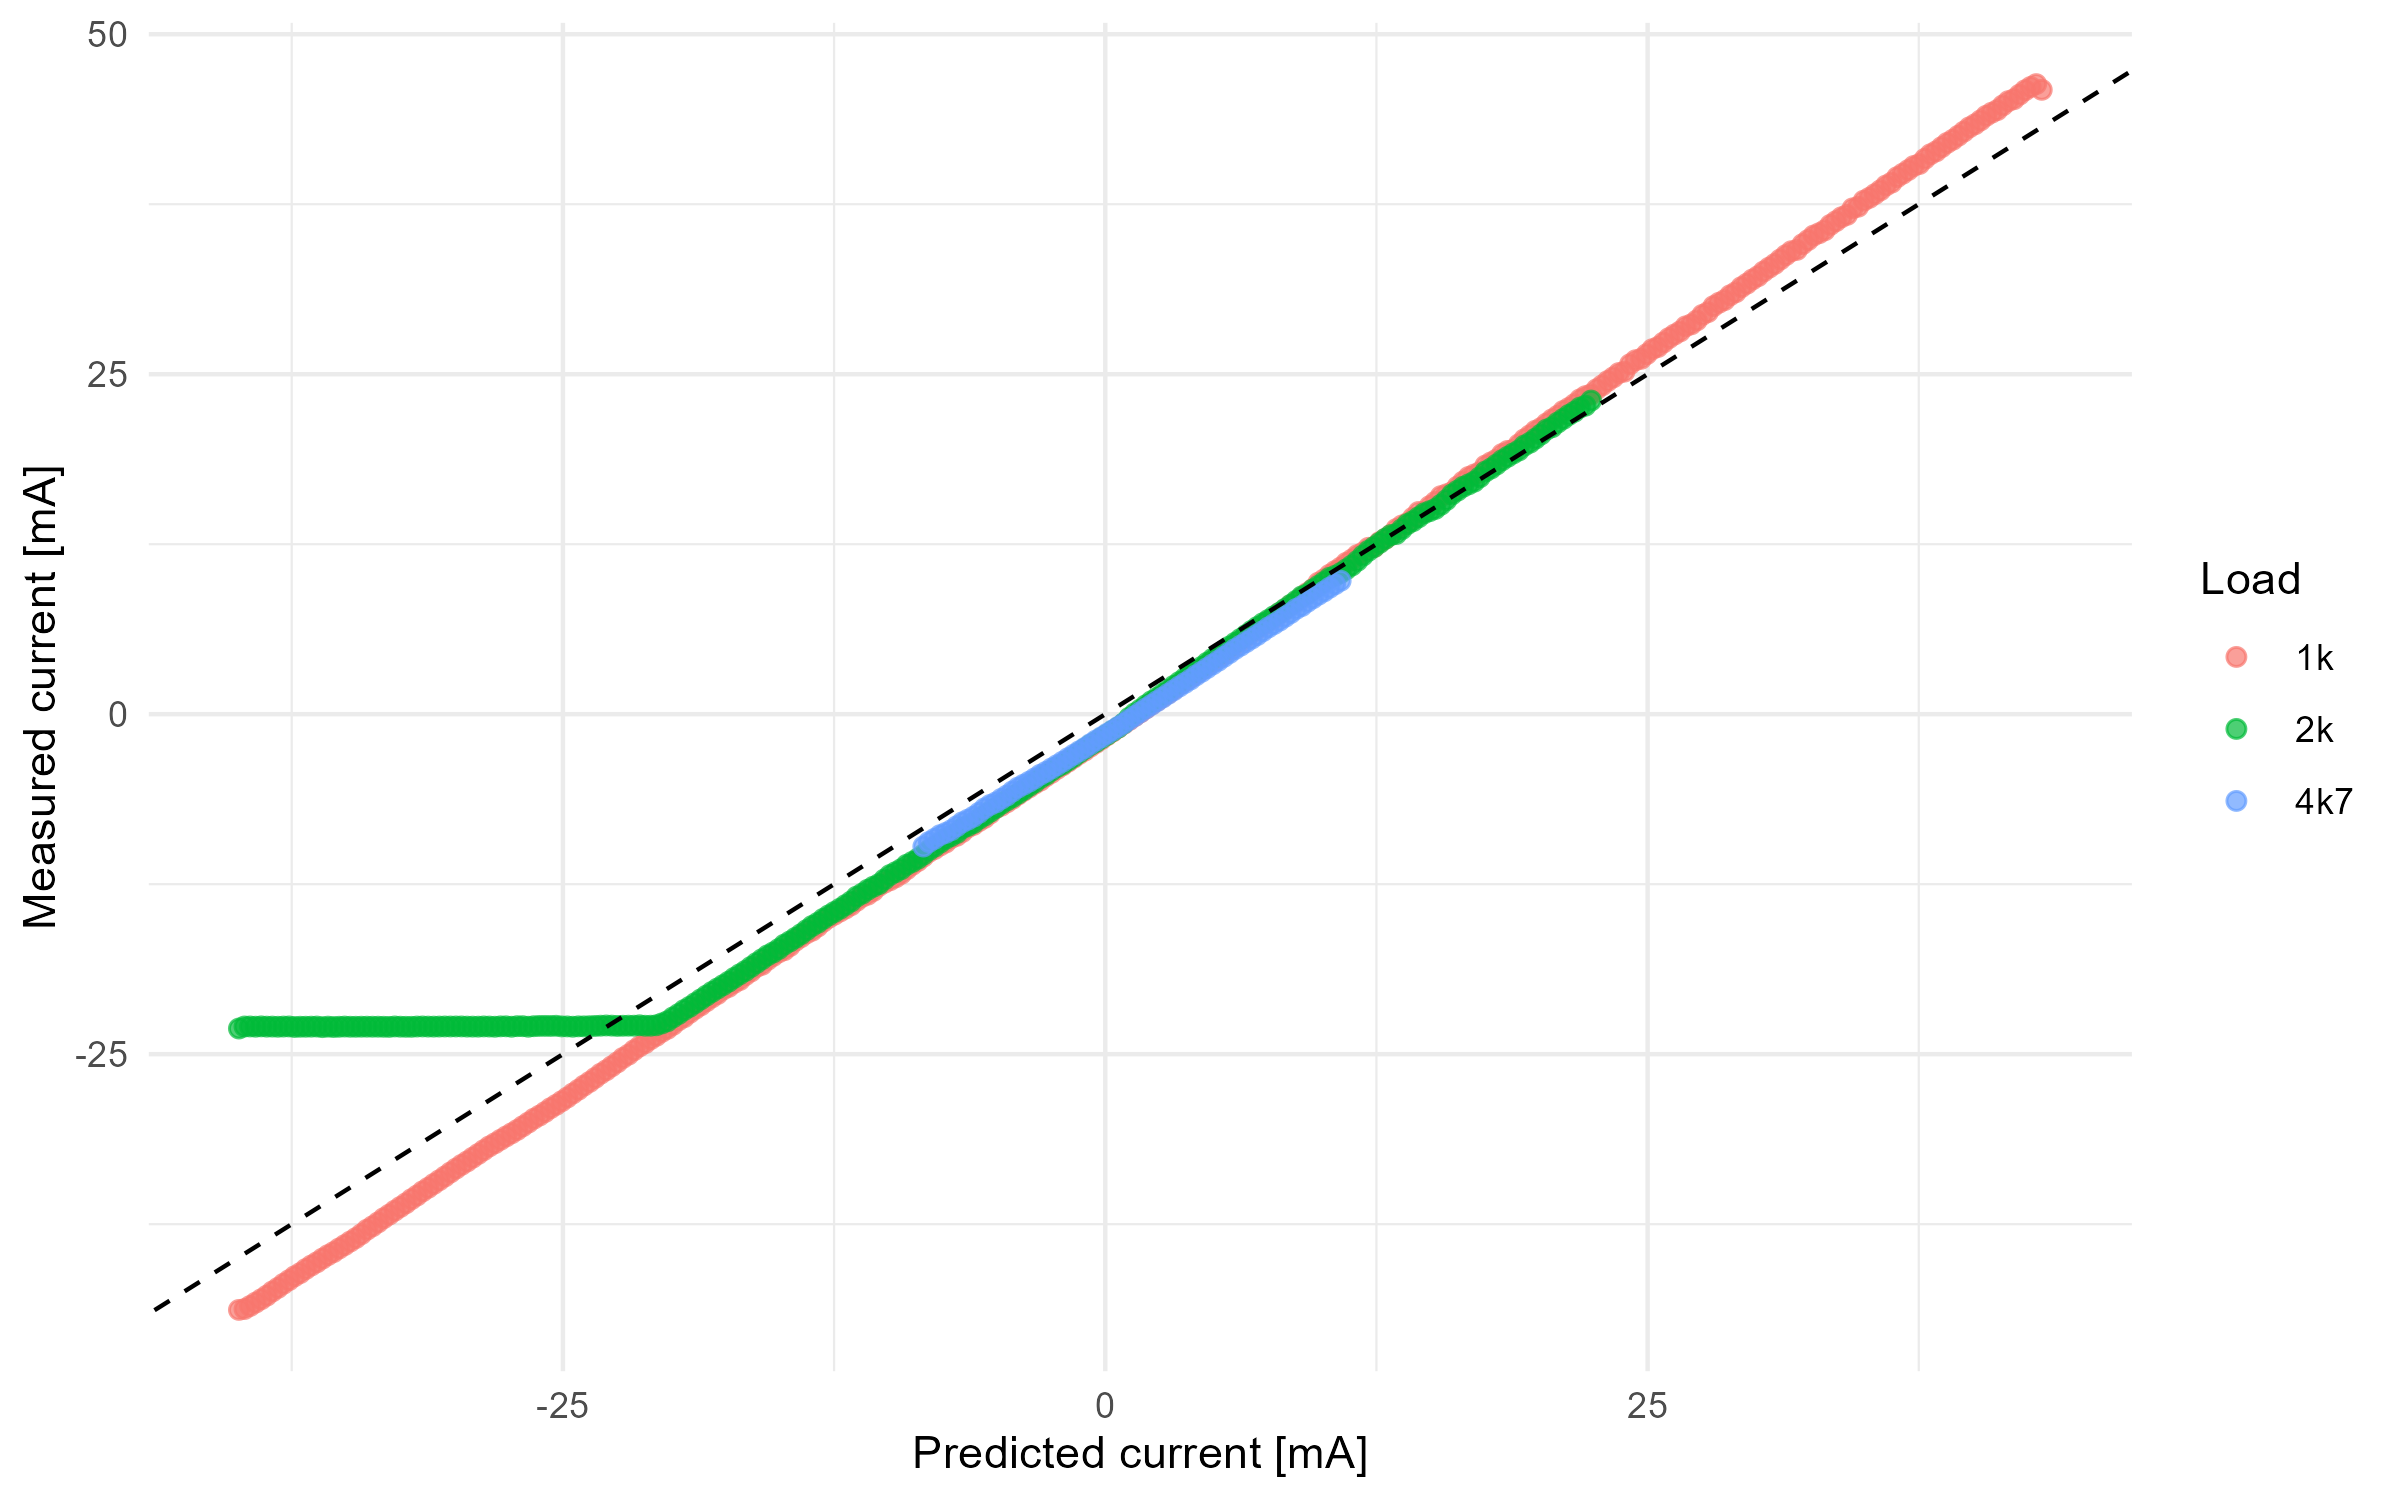
\includegraphics[width=0.74\linewidth,height=0.30\textheight,keepaspectratio]{figures/06_measured_vs_predicted.png}
\caption{Corrente medida versus corrente predita}
\end{figure}

\FloatBarrier

{\def\LTcaptype{none} % do not increment counter
\begin{longtable}[]{@{}
  >{\raggedright\arraybackslash}p{(\linewidth - 14\tabcolsep) * \real{0.1250}}
  >{\raggedright\arraybackslash}p{(\linewidth - 14\tabcolsep) * \real{0.1250}}
  >{\raggedright\arraybackslash}p{(\linewidth - 14\tabcolsep) * \real{0.1250}}
  >{\raggedright\arraybackslash}p{(\linewidth - 14\tabcolsep) * \real{0.1250}}
  >{\raggedright\arraybackslash}p{(\linewidth - 14\tabcolsep) * \real{0.1250}}
  >{\raggedright\arraybackslash}p{(\linewidth - 14\tabcolsep) * \real{0.1250}}
  >{\raggedright\arraybackslash}p{(\linewidth - 14\tabcolsep) * \real{0.1250}}
  >{\raggedright\arraybackslash}p{(\linewidth - 14\tabcolsep) * \real{0.1250}}@{}}
\toprule\noalign{}
\begin{minipage}[b]{\linewidth}\raggedright
Modelo
\end{minipage} & \begin{minipage}[b]{\linewidth}\raggedright
R2
\end{minipage} & \begin{minipage}[b]{\linewidth}\raggedright
R2 ajustado
\end{minipage} & \begin{minipage}[b]{\linewidth}\raggedright
Desvio residual (mA)
\end{minipage} & \begin{minipage}[b]{\linewidth}\raggedright
Amostras
\end{minipage} & \begin{minipage}[b]{\linewidth}\raggedright
MAE (mA)
\end{minipage} & \begin{minipage}[b]{\linewidth}\raggedright
RMSE (mA)
\end{minipage} & \begin{minipage}[b]{\linewidth}\raggedright
Erro absoluto máximo (mA)
\end{minipage} \\
\midrule\noalign{}
\endhead
\bottomrule\noalign{}
\endlastfoot
Modelo global & 0.999661 & 0.999661 & 0.389648 & 566 &
0.331486 & 0.388959 & 0.934792 \\
\midrule
Influência carga-DAC & 0.999813 & 0.999811 & 0.290484
& 566 & 0.223411 & 0.288941 & 0.743690 \\
\midrule
Modelo da carga de 1 kOhm & 0.999818 & 0.999817 & 0.354077 & 322 & 0.287084 & 0.352975 &
0.743690 \\
\midrule
Modelo da carga de 2 kOhm & 0.999794 & 0.999792 & 0.193410 & 168 & 0.159041 & 0.192255 &
0.445245 \\
\midrule
Modelo da carga de 4,7 kOhm & 0.999630 & 0.999625 & 0.111824 & 76 & 0.095924 & 0.110343 &
0.252044 \\
\end{longtable}
}
\tablecaptionbelow{Métricas de erro de predição dos modelos avaliados}

Os resultados mostram que todos os ajustes apresentam alto poder
explicativo dentro da região linear, com \(R^2\) superior a 0,999. Ainda
assim, a comparação entre os erros revela diferenças importantes. O modelo
global apresenta MAE de 0,3315 mA e RMSE de 0,3890 mA, indicando que, em
média, suas previsões se afastam da corrente medida por algumas décimas de
miliampere. O ajuste com influência da carga reduz esses erros para MAE de
0,2234 mA e RMSE de 0,2889 mA, mostrando que considerar a carga no modelo
melhora a predição sem abandonar a estrutura linear.

O erro absoluto máximo também diminui de 0,9348 mA no modelo global para
0,7437 mA no ajuste com influência da carga. Essa redução é coerente com a análise
do tópico anterior: ao permitir pequenas diferenças de intercepto e
inclinação entre as cargas, o modelo com influência da carga consegue acompanhar
melhor os dados experimentais. A Figura 10 reforça essa leitura
visualmente, pois os pontos se concentram próximos da reta de concordância
entre corrente medida e corrente predita. Assim, o erro de predição é
baixo para todos os modelos, mas o ajuste com influência da carga é o mais adequado
quando o objetivo é descrever com maior fidelidade o comportamento
experimental das três cargas.

\FloatBarrier

\section{Diagnóstico dos resíduos}\label{diagnuxf3stico-dos-resuxedduos}

O resíduo de uma observação é a diferença entre a corrente medida e a
corrente prevista pelo modelo, conforme a Equação~\ref{eq:residual}:
\begin{equation}
e_i = I_i - \hat{I}_i.
\label{eq:residual}
\end{equation}
Assim, resíduos próximos de zero indicam que o modelo reproduz bem os
valores observados. Além da magnitude dos resíduos, também é importante
avaliar sua estrutura. Em um modelo linear bem ajustado, espera-se que os
resíduos não apresentem tendência sistemática em função da variável
explicativa, tenham média próxima de zero e não mostrem padrões evidentes.
Quando os resíduos apresentam tendência, assimetria ou variância não
constante, isso não invalida automaticamente o modelo, mas indica que
algumas inferências estatísticas podem exigir cautela.

Neste tópico, os resíduos do modelo global foram avaliados porque esse é
o modelo mais simples e de maior interesse operacional. A análise permite
verificar se a aproximação por uma única reta deixa erros pequenos e
aleatórios ou se ainda existem padrões associados ao comando de DAC.

{\def\LTcaptype{none} % do not increment counter
\begin{longtable}[]{@{}
  >{\raggedright\arraybackslash}p{(\linewidth - 18\tabcolsep) * \real{0.1000}}
  >{\raggedright\arraybackslash}p{(\linewidth - 18\tabcolsep) * \real{0.1000}}
  >{\raggedright\arraybackslash}p{(\linewidth - 18\tabcolsep) * \real{0.1000}}
  >{\raggedright\arraybackslash}p{(\linewidth - 18\tabcolsep) * \real{0.1000}}
  >{\raggedright\arraybackslash}p{(\linewidth - 18\tabcolsep) * \real{0.1000}}
  >{\raggedright\arraybackslash}p{(\linewidth - 18\tabcolsep) * \real{0.1000}}
  >{\raggedright\arraybackslash}p{(\linewidth - 18\tabcolsep) * \real{0.1000}}
  >{\raggedright\arraybackslash}p{(\linewidth - 18\tabcolsep) * \real{0.1000}}
  >{\raggedright\arraybackslash}p{(\linewidth - 18\tabcolsep) * \real{0.1000}}
  >{\raggedright\arraybackslash}p{(\linewidth - 18\tabcolsep) * \real{0.1000}}@{}}
\toprule\noalign{}
\begin{minipage}[b]{\linewidth}\raggedright
\textbf{Modelo}
\end{minipage} & \begin{minipage}[b]{\linewidth}\raggedright
\textbf{Média dos resíduos (mA)}
\end{minipage} & \begin{minipage}[b]{\linewidth}\raggedright
\textbf{Desvio dos resíduos (mA)}
\end{minipage} & \begin{minipage}[b]{\linewidth}\raggedright
\textbf{Mediana dos resíduos (mA)}
\end{minipage} & \begin{minipage}[b]{\linewidth}\raggedright
\textbf{Resíduo mínimo (mA)}
\end{minipage} & \begin{minipage}[b]{\linewidth}\raggedright
\textbf{Resíduo máximo (mA)}
\end{minipage} & \begin{minipage}[b]{\linewidth}\raggedright
\textbf{MAE (mA)}
\end{minipage} & \begin{minipage}[b]{\linewidth}\raggedright
\textbf{RMSE (mA)}
\end{minipage} & \begin{minipage}[b]{\linewidth}\raggedright
\textbf{Amostras no Shapiro}
\end{minipage} & \begin{minipage}[b]{\linewidth}\raggedright
\textbf{Valor-p Shapiro}
\end{minipage} \\
\midrule\noalign{}
\endhead
\bottomrule\noalign{}
\endlastfoot
Modelo global & 0 & 0.389303 & 0.015381 & -0.934792 &
0.738906 & 0.331486 & 0.388959 & 566 & \(<0{,}001\) \\
\end{longtable}
}
\tablecaptionbelow{Resumo dos resíduos do modelo global e teste de normalidade}

A média dos resíduos é praticamente nula, como esperado em um ajuste por
mínimos quadrados. Isso indica ausência de viés médio global: considerando
todo o conjunto de dados, o modelo não tende claramente a superestimar ou
subestimar a corrente. A mediana dos resíduos, igual a 0,0154 mA, também
fica muito próxima de zero, reforçando que o centro da distribuição dos
erros está próximo do valor esperado.

A dispersão dos resíduos, entretanto, mostra a magnitude prática do erro.
O desvio dos resíduos é 0,3893 mA, o MAE é 0,3315 mA e o RMSE é
0,3890 mA. Como o RMSE penaliza mais erros maiores, sua proximidade em
relação ao desvio residual indica que os erros são pequenos, mas ainda há
alguns desvios mais pronunciados. Isso também aparece nos extremos: o
maior erro negativo é -0,9348 mA e o maior erro positivo é 0,7389 mA. Em
termos práticos, esses valores definem a ordem de grandeza do erro
esperado ao usar o modelo global dentro da região linear.

O teste de Shapiro-Wilk avalia a compatibilidade dos resíduos com uma
distribuição normal. A hipótese nula desse teste é que os resíduos seguem
distribuição normal. Como o p-valor é inferior a 0,001, rejeita-se essa
hipótese ao nível de significância de 5\%. Portanto, a normalidade dos
resíduos é questionável. Esse resultado não impede o uso do modelo como
aproximação preditiva, mas sugere cautela ao interpretar testes e
intervalos que dependem fortemente da suposição de normalidade dos erros.

\begin{figure}
\centering
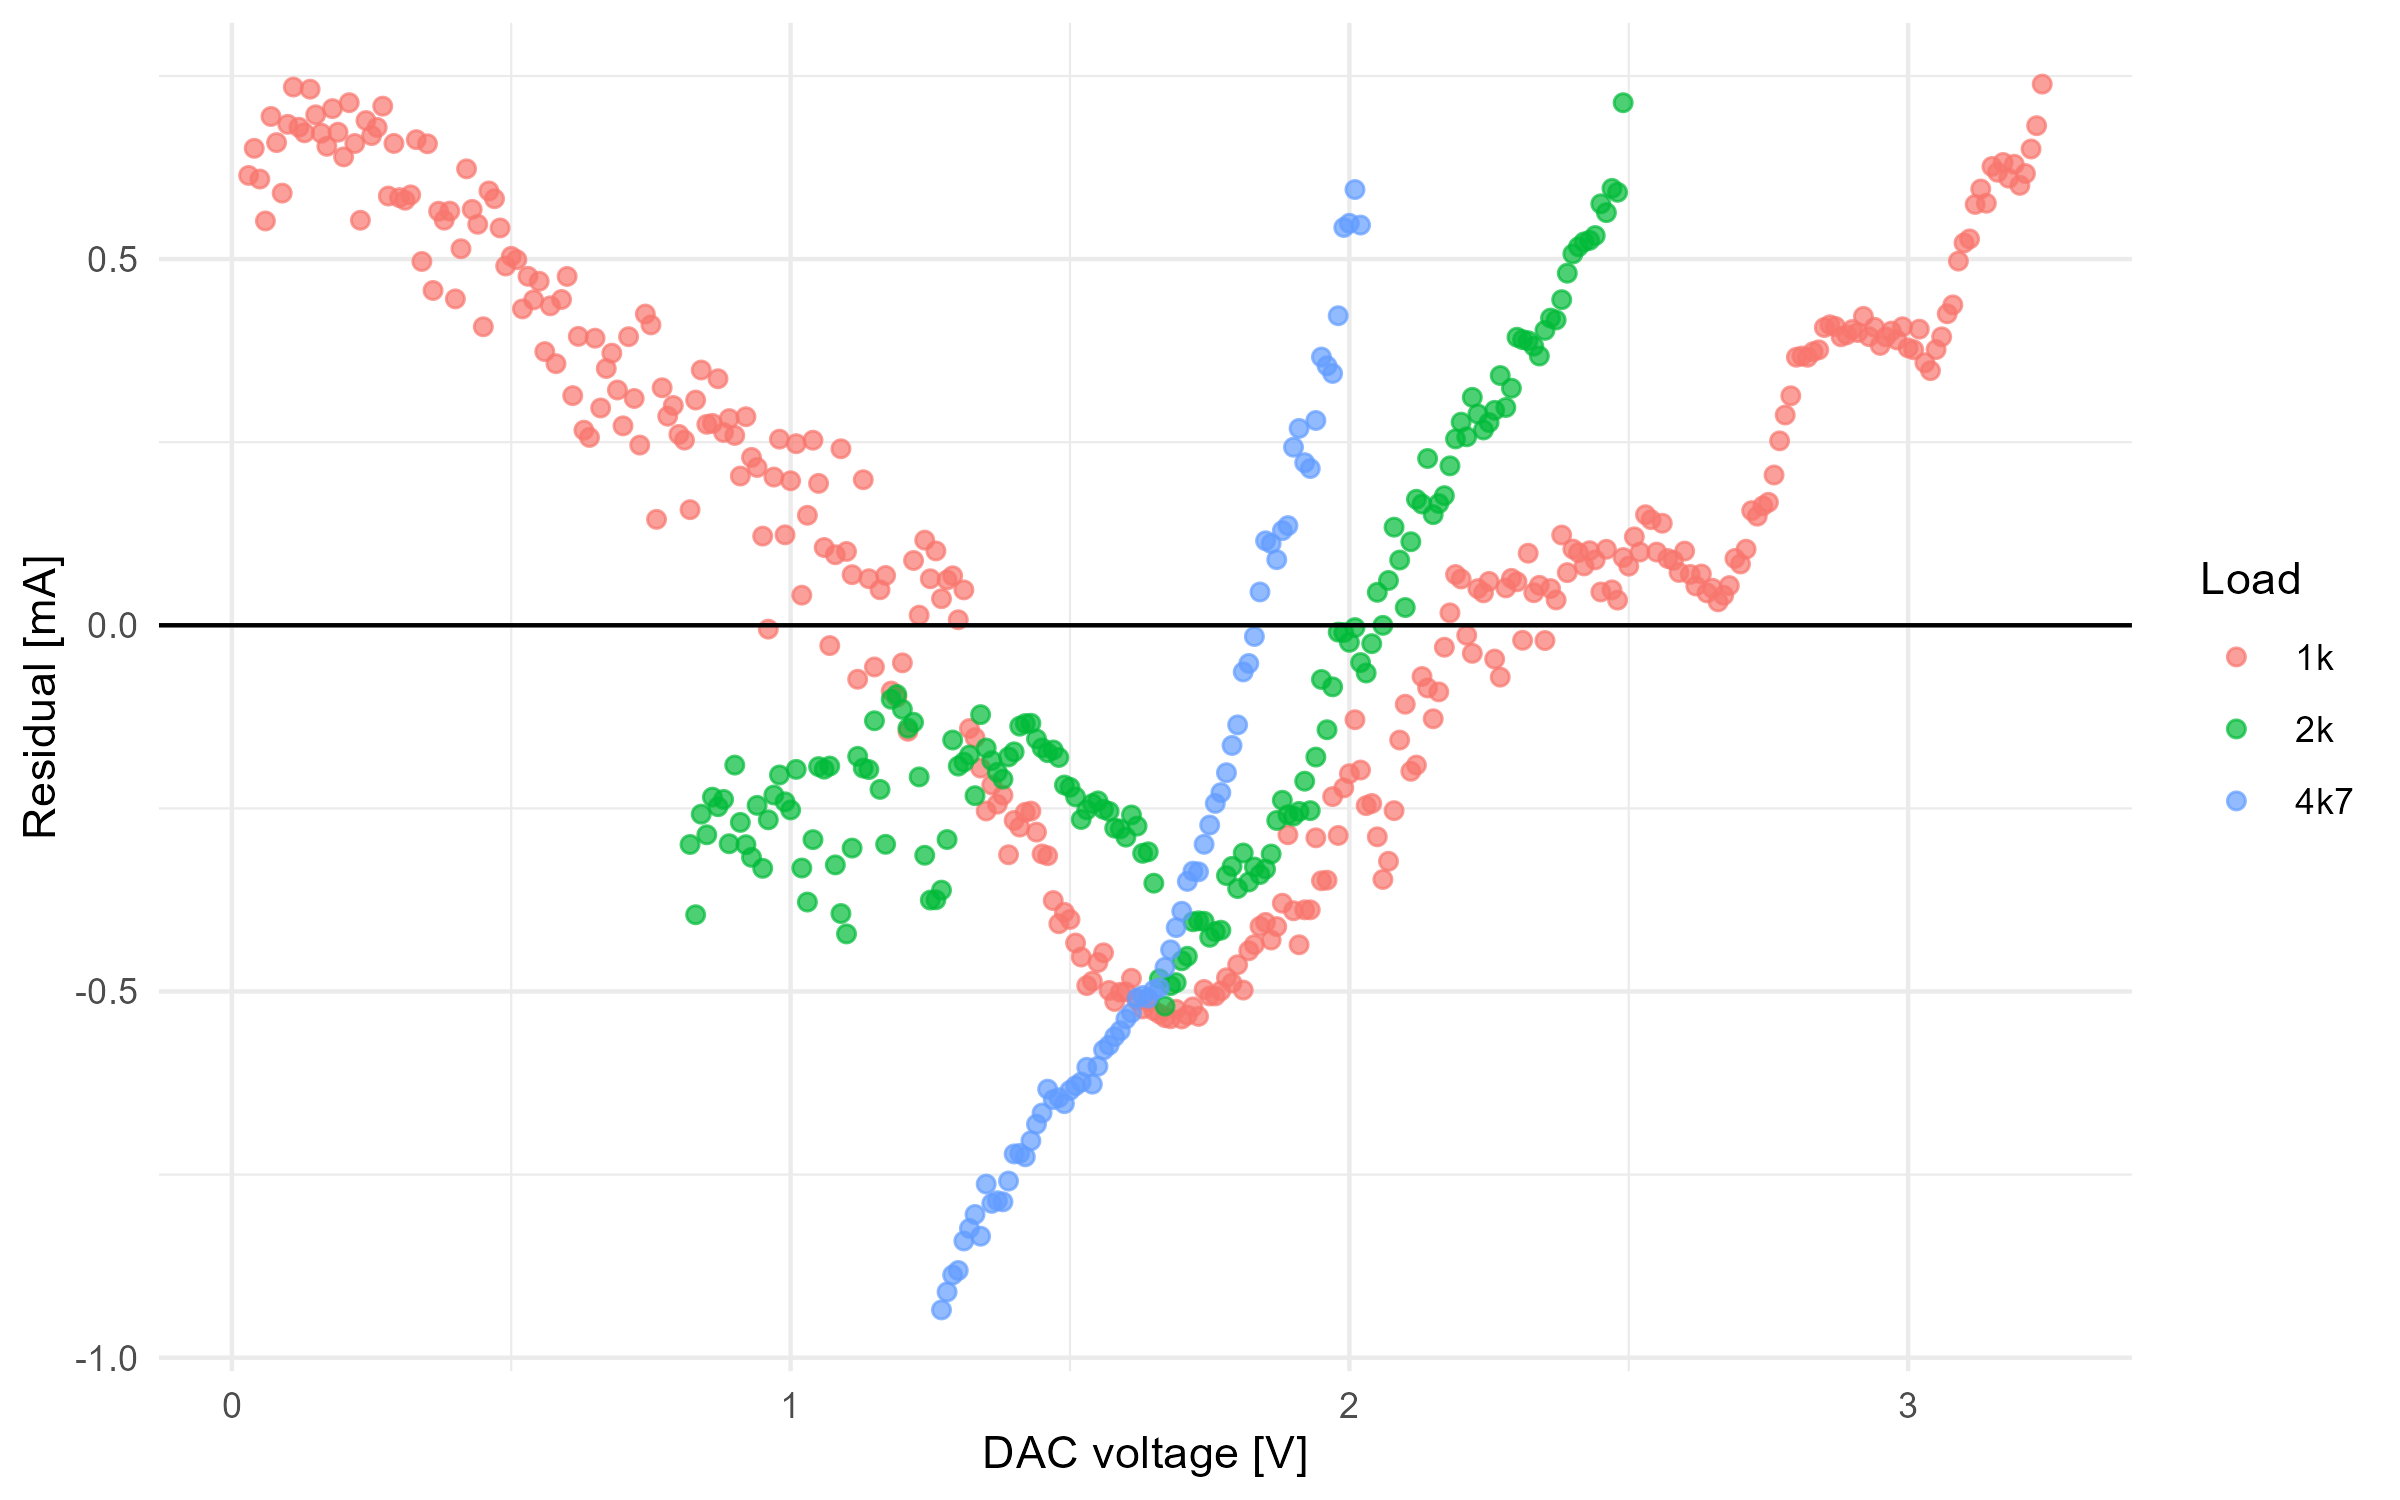
\includegraphics[width=0.76\linewidth,height=0.34\textheight,keepaspectratio]{figures/09_residuals_vs_dac.png}
\caption{Resíduos em função do DAC}
\end{figure}

Na Figura 11, a análise visual complementa a tabela. Se os resíduos
fossem puramente aleatórios em torno de zero, seria esperado observar uma
nuvem de pontos sem tendência clara ao longo do comando de DAC. A presença
de estrutura visual ou agrupamentos indica que o erro do modelo não é
completamente aleatório, o que é coerente com os resultados posteriores de
heterocedasticidade e validação por blocos. Assim, o modelo global descreve bem
a tendência média entre DAC e corrente, mas os resíduos mostram que ainda
há informação sistemática não capturada por uma única reta média.

\FloatBarrier
\clearpage

\section{Homocedasticidade}\label{homocedasticidade}

A homocedasticidade é a condição em que a variância dos resíduos permanece
aproximadamente constante ao longo da faixa de valores preditos ou da
variável explicativa. Em regressão linear, essa condição é importante
porque muitos resultados inferenciais, como erros padrão, intervalos de
confiança e testes de significância, assumem que os resíduos têm dispersão
semelhante em toda a faixa analisada.

Quando a variância dos resíduos muda ao longo da escala de DAC ou da
corrente prevista, ocorre heterocedasticidade. Nesse caso, o modelo ainda
pode representar bem a tendência média, mas a incerteza das previsões pode
ser diferente em regiões distintas da curva. Para avaliar essa condição,
foi aplicado o teste de Breusch-Pagan. A hipótese nula do teste é
apresentada na Equação~\ref{eq:bp-h0}:
\begin{equation}
H_0: \text{a variância dos resíduos é constante}.
\label{eq:bp-h0}
\end{equation}
A hipótese alternativa é apresentada na Equação~\ref{eq:bp-h1}:
\begin{equation}
H_1: \text{a variância dos resíduos não é constante}.
\label{eq:bp-h1}
\end{equation}

{\def\LTcaptype{none} % do not increment counter
\begin{longtable}[]{@{}
  >{\raggedright\arraybackslash}p{(\linewidth - 6\tabcolsep) * \real{0.2800}}
  >{\raggedright\arraybackslash}p{(\linewidth - 6\tabcolsep) * \real{0.2000}}
  >{\raggedright\arraybackslash}p{(\linewidth - 6\tabcolsep) * \real{0.1800}}
  >{\raggedright\arraybackslash}p{(\linewidth - 6\tabcolsep) * \real{0.3400}}@{}}
\toprule\noalign{}
\begin{minipage}[b]{\linewidth}\raggedright
\textbf{Teste}
\end{minipage} & \begin{minipage}[b]{\linewidth}\raggedright
\textbf{Estatística}
\end{minipage} & \begin{minipage}[b]{\linewidth}\raggedright
\textbf{Valor-p}
\end{minipage} & \begin{minipage}[b]{\linewidth}\raggedright
\textbf{Interpretação}
\end{minipage} \\
\midrule\noalign{}
\endhead
\bottomrule\noalign{}
\endlastfoot
Breusch-Pagan & 27.838682 & \(<0{,}001\) &
Evidência de variância residual não constante \\
\end{longtable}
}
\tablecaptionbelow{Teste de homocedasticidade dos resíduos}

O teste apresenta estatística de 27,8387 e p-valor inferior a 0,001.
Como esse p-valor é menor que o nível de significância de 5\%, rejeita-se
\(H_0\). Portanto, há evidência estatística de heterocedasticidade, isto é,
a variância dos resíduos não pode ser considerada constante ao longo da
faixa analisada.

Esse resultado deve ser interpretado em conjunto com os demais tópicos. A
heterocedasticidade não significa que a relação linear entre DAC e
corrente esteja errada; significa que a dispersão dos erros não é
uniforme. Assim, o modelo global continua útil como aproximação média, mas
os intervalos de confiança, os p-valores clássicos e a incerteza associada
às previsões devem ser lidos com cautela.

\section{Validação cruzada por
blocos}\label{validauxe7uxe3o-cruzada-por-blocos}

A validação por blocos usa cinco blocos contíguos ordenados, treinando
em quatro blocos e testando no bloco remanescente. Isso evita usar
apenas uma validação aleatória que mistura pontos vizinhos da rampa.

A validação cruzada é usada para avaliar a capacidade de generalização do
modelo, isto é, seu desempenho em dados que não foram usados diretamente
no ajuste. Neste estudo, uma divisão aleatória simples poderia produzir
uma avaliação otimista, porque pontos vizinhos da rampa são muito
semelhantes entre si. Se amostras quase consecutivas fossem separadas
aleatoriamente entre treino e teste, o conjunto de teste ficaria muito
parecido com o conjunto de treino.

Por esse motivo, foi usada validação cruzada por blocos contíguos. Em vez
de embaralhar os dados, a sequência é dividida em cinco blocos ordenados.
Em cada rodada, quatro blocos são usados para treinamento e um bloco é
usado para teste. Essa estratégia é mais conservadora para dados obtidos
em rampa, pois avalia o modelo em segmentos inteiros da aquisição.

{\def\LTcaptype{none} % do not increment counter
\begin{longtable}[]{@{}
  >{\raggedright\arraybackslash}p{(\linewidth - 10\tabcolsep) * \real{0.1667}}
  >{\raggedright\arraybackslash}p{(\linewidth - 10\tabcolsep) * \real{0.1667}}
  >{\raggedright\arraybackslash}p{(\linewidth - 10\tabcolsep) * \real{0.1667}}
  >{\raggedright\arraybackslash}p{(\linewidth - 10\tabcolsep) * \real{0.1667}}
  >{\raggedright\arraybackslash}p{(\linewidth - 10\tabcolsep) * \real{0.1667}}
  >{\raggedright\arraybackslash}p{(\linewidth - 10\tabcolsep) * \real{0.1667}}@{}}
\toprule\noalign{}
\begin{minipage}[b]{\linewidth}\raggedright
\textbf{Bloco}
\end{minipage} & \begin{minipage}[b]{\linewidth}\raggedright
\textbf{Amostras de treino}
\end{minipage} & \begin{minipage}[b]{\linewidth}\raggedright
\textbf{Amostras de teste}
\end{minipage} & \begin{minipage}[b]{\linewidth}\raggedright
\textbf{MAE (mA)}
\end{minipage} & \begin{minipage}[b]{\linewidth}\raggedright
\textbf{RMSE (mA)}
\end{minipage} & \begin{minipage}[b]{\linewidth}\raggedright
\textbf{Erro absoluto máximo (mA)}
\end{minipage} \\
\midrule\noalign{}
\endhead
\bottomrule\noalign{}
\endlastfoot
1 & 452 & 114 & 1.094951 & 1.149833 & 1.640076 \\
\midrule
2 & 453 & 113 & 0.336214 & 0.391106 & 0.604763 \\
\midrule
3 & 453 & 113 & 0.614323 & 0.672667 & 1.249332 \\
\midrule
4 & 453 & 113 & 0.287021 & 0.314989 & 0.575789 \\
\midrule
5 & 453 & 113 & 0.469936 & 0.525130 & 0.978239 \\
\end{longtable}
}
\tablecaptionbelow{Erros de validação cruzada por bloco}

Os erros por bloco não são idênticos, o que indica que o desempenho do
modelo varia ao longo da faixa de aquisição. O bloco 1 apresenta o maior
erro, com MAE de 1,0950 mA, RMSE de 1,1498 mA e erro absoluto máximo de
1,6401 mA. Esse comportamento sugere que esse segmento da rampa é mais
difícil de prever pelo modelo ajustado com os demais blocos. Nos blocos 2
a 5, os erros são menores, com RMSE variando aproximadamente de 0,3150 mA
a 0,6727 mA.

{\def\LTcaptype{none} % do not increment counter
\begin{longtable}[]{@{}
  >{\raggedright\arraybackslash}p{(\linewidth - 12\tabcolsep) * \real{0.1429}}
  >{\raggedright\arraybackslash}p{(\linewidth - 12\tabcolsep) * \real{0.1429}}
  >{\raggedright\arraybackslash}p{(\linewidth - 12\tabcolsep) * \real{0.1429}}
  >{\raggedright\arraybackslash}p{(\linewidth - 12\tabcolsep) * \real{0.1429}}
  >{\raggedright\arraybackslash}p{(\linewidth - 12\tabcolsep) * \real{0.1429}}
  >{\raggedright\arraybackslash}p{(\linewidth - 12\tabcolsep) * \real{0.1429}}
  >{\raggedright\arraybackslash}p{(\linewidth - 12\tabcolsep) * \real{0.1429}}@{}}
\toprule\noalign{}
\begin{minipage}[b]{\linewidth}\raggedright
\textbf{Blocos}
\end{minipage} & \begin{minipage}[b]{\linewidth}\raggedright
\textbf{RMSE médio (mA)}
\end{minipage} & \begin{minipage}[b]{\linewidth}\raggedright
\textbf{Desvio do RMSE (mA)}
\end{minipage} & \begin{minipage}[b]{\linewidth}\raggedright
\textbf{MAE médio (mA)}
\end{minipage} & \begin{minipage}[b]{\linewidth}\raggedright
\textbf{Desvio do MAE (mA)}
\end{minipage} & \begin{minipage}[b]{\linewidth}\raggedright
\textbf{Erro máx. médio (mA)}
\end{minipage} & \begin{minipage}[b]{\linewidth}\raggedright
\textbf{Desvio do erro máx. (mA)}
\end{minipage} \\
\midrule\noalign{}
\endhead
\bottomrule\noalign{}
\endlastfoot
5 & 0.610745 & 0.330716 & 0.560489 & 0.324743 & 1.00964 & 0.449455 \\
\end{longtable}
}
\tablecaptionbelow{Resumo agregado da validação cruzada por blocos}

No resumo agregado, o RMSE médio é 0,6107 mA e o MAE médio é 0,5605 mA.
Esses valores são maiores que os erros obtidos quando o modelo é avaliado
nos próprios dados usados no ajuste, o que é esperado em validação
cruzada. A validação por blocos fornece uma estimativa mais realista da
capacidade preditiva fora do conjunto de treino.

\begin{figure}
\centering
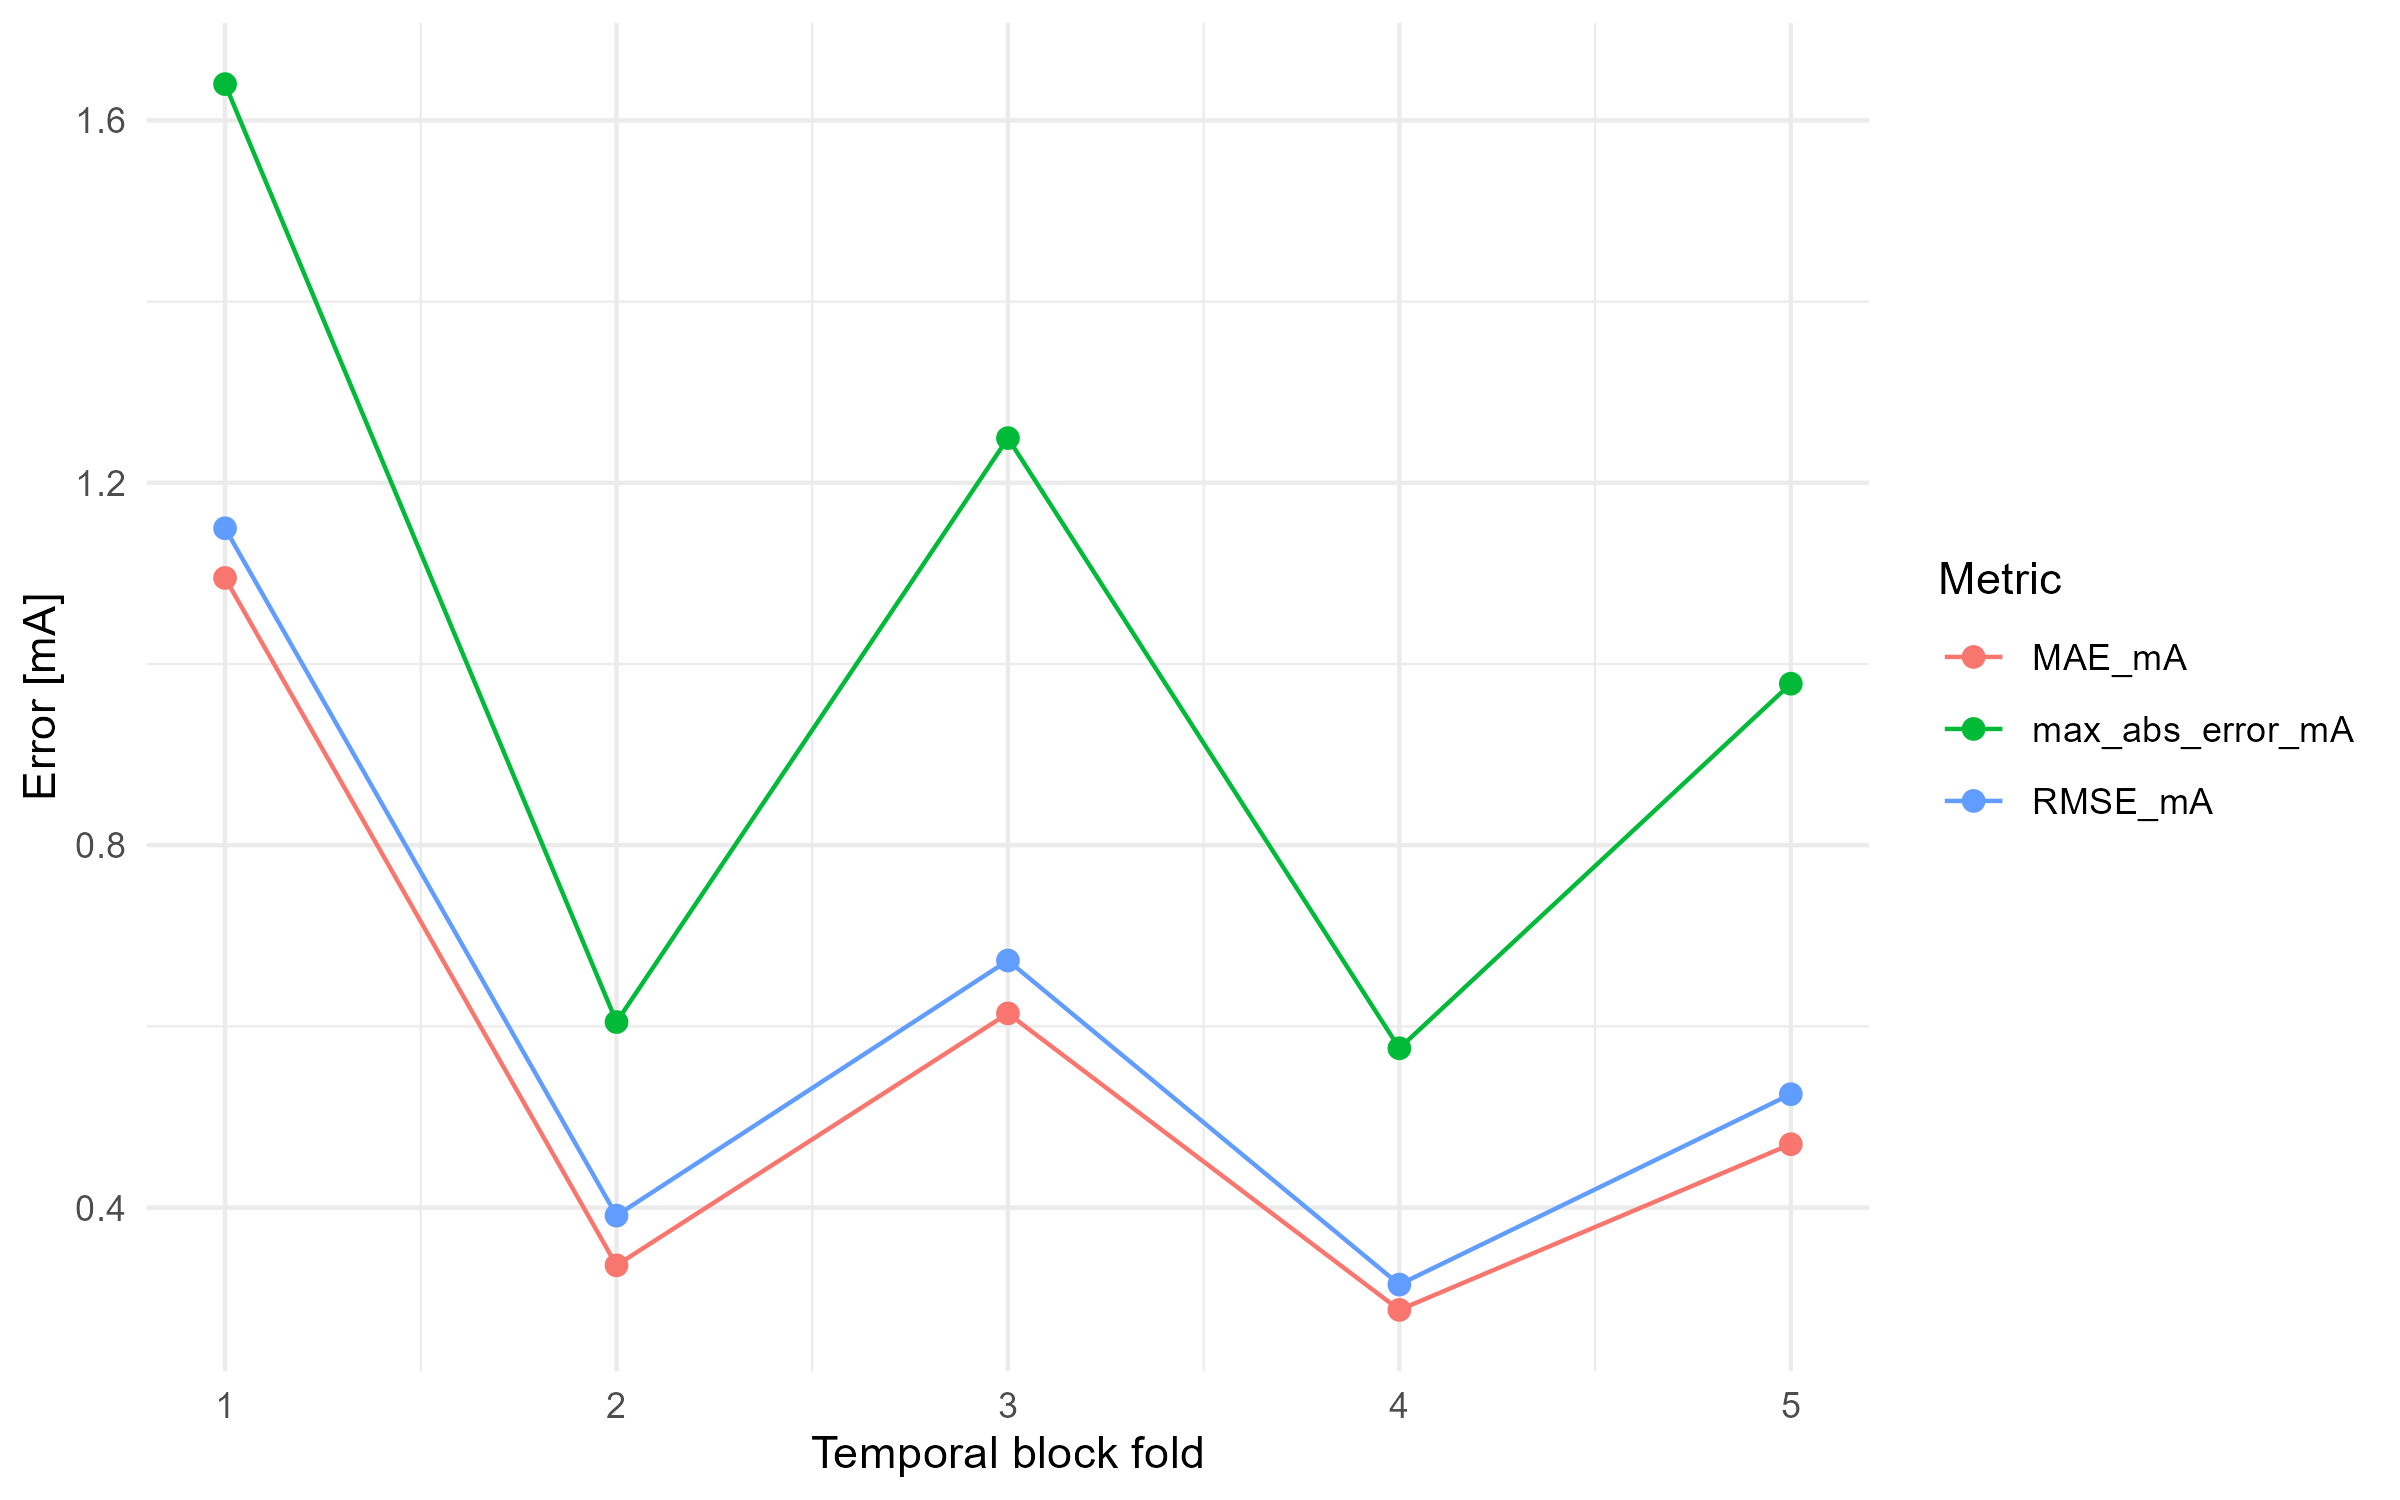
\includegraphics[width=0.78\linewidth,height=0.34\textheight,keepaspectratio]{figures/15_block_cross_validation_errors.png}
\caption{Erros da validação cruzada por blocos}
\end{figure}

A figura de validação cruzada evidencia a diferença de desempenho entre os blocos. O
primeiro bloco concentra os maiores erros, enquanto os blocos centrais e
finais apresentam desempenho mais estável. Isso indica que o modelo possui
boa capacidade preditiva geral dentro da região linear, mas sua precisão
não é perfeitamente uniforme em todos os segmentos da rampa. Essa
observação é coerente com os diagnósticos anteriores de resíduos,
heterocedasticidade e validação por blocos.

\FloatBarrier

\clearpage

\section{Conclusões}\label{conclusuxf5es}

A caracterização mostrou que a relação entre o comando de DAC e a corrente
de saída pode ser descrita com alta precisão por modelos lineares dentro
da região comum de compliance. Nessa faixa, as correlações são muito
próximas de -1, os coeficientes angulares são estatisticamente
significativos e os erros de predição permanecem baixos. Portanto, para a
região linear identificada, o comportamento do estágio de saída é
previsível e pode ser modelado de forma simples.

O modelo global, baseado em uma única reta para todas as cargas, é útil
como aproximação operacional. Ele resume a tendência média do sistema e
fornece uma descrição compacta da relação entre tensão de DAC e corrente.
Entretanto, a comparação por ANOVA/teste F mostrou que o ajuste com
influência da carga sobre a relação DAC-corrente reduz significativamente a soma dos
quadrados residual. Isso indica que pequenas diferenças de intercepto e
inclinação entre as cargas existem e melhoram a descrição estatística dos
dados.

As métricas de predição confirmam essa leitura. O modelo global já
apresenta erro médio baixo, mas o ajuste com influência da carga reduz MAE, RMSE e
erro absoluto máximo. Assim, quando o objetivo é uma aproximação simples,
o modelo global é suficiente; quando o objetivo é descrever com maior
fidelidade o comportamento experimental das três cargas, o modelo com
influência da carga é mais adequado.

Os diagnósticos também delimitam o alcance das conclusões. A análise dos
resíduos indica que o modelo global não apresenta viés médio relevante,
mas a normalidade dos resíduos é questionável. Além disso, o teste de
Breusch-Pagan indica heterocedasticidade, ou seja, a dispersão dos erros
não é constante em toda a faixa analisada. Portanto, os modelos são
adequados como descrição empírica e ferramenta de predição dentro da
região linear, mas a interpretação inferencial deve ser feita com cautela.

Fora da região linear, a limitação de compliance passa a dominar o
comportamento. Isso não representa necessariamente uma falha do estágio,
mas define um limite operacional importante: à medida que a carga aumenta,
a faixa de corrente útil diminui. Como a arquitetura é open-loop, o
firmware não detecta automaticamente quando o estágio entra em saturação e
a corrente entregue deixa de acompanhar a corrente prevista pelo modelo.
Uma melhoria natural seria incluir realimentação de corrente, monitoramento
de compliance ou outra forma de operação em malha fechada.

\clearpage

\section*{Referências}\label{referuxeancias}
\addcontentsline{toc}{section}{Referências}

{[}1{]} Tiago de Paula Silva, ``Experimental Characterization of the
Output Stage of a Functional Electrical Stimulator Based on a Howland
Current Source,'' artigo produzido no contexto da disciplina PEL309,
Centro Universitário FEI, 2026.

{[}2{]} Tiago de Paula Silva, ``FEI - PME406: script R da análise
estatística,'' repositório GitHub. Disponível em:
\url{https://github.com/import-tiago/FEI/blob/main/MSc/PME406/1.Analysis/analise_rstudio.R}.

{[}3{]} Tiago de Paula Silva, ``FEI - PME406: dados brutos em CSV
exportados do osciloscópio,'' repositório GitHub. Arquivos
\texttt{1k.csv}, \texttt{2k.csv} e \texttt{4k7.csv}. Disponível em:
\url{https://github.com/import-tiago/FEI/tree/main/MSc/PME406/0.Data}.

\end{document}
